\documentclass[class=article, crop=false, 12pt]{standalone}
\usepackage[subpreambles=true]{standalone}
\usepackage{../.common/common}


\author{Tony Shing}
%\pretitle{Supplementary}

\topic{T11 (Electromagnetism)}
\title{Electrostatics}

\version{2025} % leave blank for omitting

\begin{document}

\maketitle


\begin{overview}
    \begin{itemize}
        \item Basic problems: Find $\vvec{E}$ and $V$ by Coulomb's law with integration
        \item Gauss law, electric flux, divergence \& divergence theorem
        \item Electrical potential \& Poisson equation
        \item Image charge method
    \end{itemize}


\end{overview}

\vskip 1em
In electromagnetism, 
theoretically every problem can be solved through a set of PDEs
called the \bf{Maxwell Equations}.\\[-2em]
\begin{center}
    \begin{minipage}{0.3\textwidth}
        \aleq{
            \tkn{maxwell_gauss}{\div} \vvec{E} &= \frac{\rho}{\epsilon_0}\\
            \curl \vvec{E} &= -\pdvv{\vvec{B}}{t}
        }
    \end{minipage}
    \hspace{0.05\textwidth}
    \begin{minipage}{0.3\textwidth}
        \aleq{
            \div \vvec{B} &= 0\\
            \curl \vvec{B} &= \mu_0 \vvec{J} + \mu_0\epsilon_0\pdvv{\vvec{E}}{t}
        }
    \end{minipage}
\end{center}
\addArrow[blue]{maxwell_gauss}{(-5ex,0)}{}{(-3ex,1ex)}

However, a \it{system of PDEs} is too complicated to be solved.
So we need to learn different "tricks" to avoid them,
which are enough for some simple scenarios.\\

Electrostatics only concerns the \nth{1} equation of the set - \cul[blue]{Gauss's law}. 




\linesep
% content begins here
% Section %%%%%%%%%%%%%%%%%%%%%%%%%%%%%%%%%%%%%%%%%%%%%%%%%%%%
\section{Coulomb's Law with Integration}

%%%%%%%%%%%%%%
\subsection{From Points to Distributions}

In high school Physics, 
problems related to electrostatics only concern point charges.
For example, given the magnitudes and positions of several point charges,
the question may ask you the E-field at one position. 

\begin{center}
    \begin{minipage}{0.2\linewidth}
        \centering
        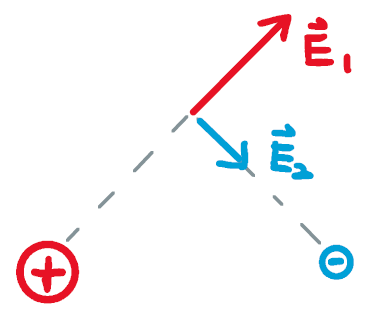
\includegraphics[width=\textwidth]{coulomb1}\\
        Given charges $Q$ (A number)
    \end{minipage}
    \qquad$\Rightarrow$\qquad
    \begin{minipage}{0.2\linewidth}
        \centering
        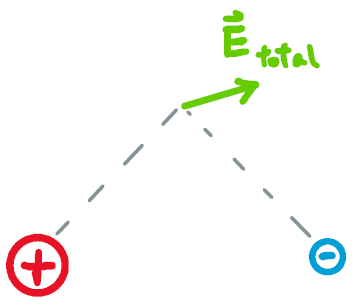
\includegraphics[width=\textwidth]{coulomb2}\\
        Ask for E-field $\vvec{E}$ (A vector)
    \end{minipage}
\end{center}

\vskip 1ex
But in university physics, we promote point charges to a charge distribution (function) in a space,
and our task becomes solving for the E-field distribution (function) in the space.

\begin{center}
    \begin{minipage}{0.4\linewidth}
        \centering
        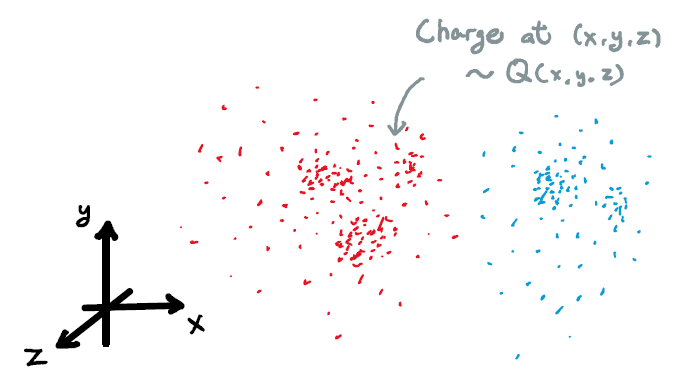
\includegraphics[width=\textwidth]{coulomb3}\\
        Given charges \bf{distribution}\\ $Q(x,y,z)$\\ (A scalar \cul[red]{function} of position)
    \end{minipage}
    \qquad$\Rightarrow$\qquad
    \begin{minipage}{0.35\linewidth}
        \centering
        \vskip 0.8em
        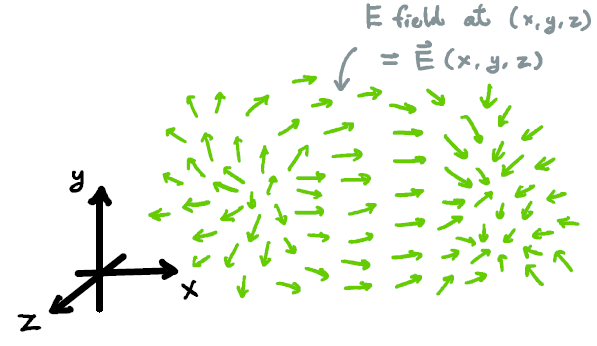
\includegraphics[width=\textwidth]{coulomb4}\\
        Ask for E-field \bf{distribution}\\ $\vvec{E}(x,y,z)$\\ (A vector \cul[red]{function} of position)
    \end{minipage}
\end{center}

\vskip 1ex
This ultimate task is to \cul[red]{find a function from another function}! 
This is why E\&M is generally a hard topic - 
these problems were supposed to be solved by PDEs!


%%%%%%%%%%%%%%
\subsection{Charge Densities}

Yet we may avoid solving PDE when the problem is simple enough.
For example, if we are only interested in the E-field at one specific point - 
we only need to carry out one or two integrations after writing down the Coulomb's law towards that point.\\

Firstly, we shall promote point charges to charge distributions.
\aleq{
    \quad\qquad\qquad \ \qty(\mstack{\text{Point}\\\text{charge}}) \ =\ Q 
    \qquad\ \xRightarrow{\phantom{000}}\qquad
    \int_{\substack{\text{whole}\\\text{space}}} \dd{Q} \quad \sim\ 
    \sum_\text{everywhere} \qty(\mstack{\text{Infinitestimal}\\\text{charge units}})
}

Because we are living in a 3D world, 
charges may be contained in objects of different dimensions. 
A charge distribution is often represented by a \bf{charge density function}.

\vskip 1em
\begin{minipage}{0.6\linewidth}
    \begin{itemize}
        \item \bf{\ul{Line Charge Density}} : $\lambda = \lambda(x)$
        \aleq{
            \quad\Rightarrow\quad \dd{Q} = \lambda\dd{l} 
            = \qty(\substack{\text{Charge}\\\text{per length}})\qty(\substack{\text{Unit}\\\text{length}})
        }
    \end{itemize}
\end{minipage}
\hspace{0.05\textwidth}
\begin{minipage}{0.18\linewidth}
    \centering
    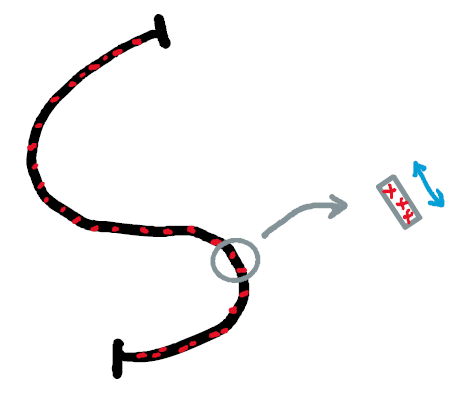
\includegraphics[width=\textwidth]{charge_line}
\end{minipage}

\vskip 1em
\begin{minipage}{0.58\linewidth}
    \begin{itemize}
        \item \bf{\ul{Surface Charge Density}} : $\sigma = \sigma(x,y)$
        \aleq{
            \ \ \Rightarrow\quad \dd{Q} = \sigma\dd{s} 
            = \qty(\substack{\text{Charge}\\\text{per area}})\qty(\substack{\text{Unit}\\\text{area}})
        }
    \end{itemize}
\end{minipage}
\hspace{0.05\textwidth}
\begin{minipage}{0.25\linewidth}
    \centering
    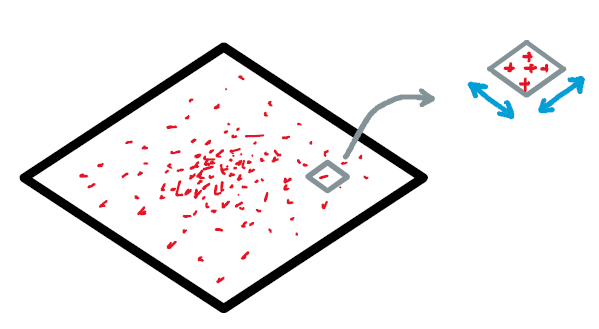
\includegraphics[width=\textwidth]{charge_sur}
\end{minipage}

\vskip 1em
\begin{minipage}{0.6\linewidth}
    \begin{itemize}
        \item \bf{\ul{Volume Charge Density}} : $\rho = \rho(x,y,z)$
        \aleq{
            \qquad\Rightarrow\quad \dd{Q} = \rho\dd{\tau} 
            = \qty(\substack{\text{Charge}\\\text{per volume}})\qty(\substack{\text{Unit}\\\text{volume}})
        }
    \end{itemize}
\end{minipage}
\hspace{0.05\textwidth}
\begin{minipage}{0.25\linewidth}
    \centering
    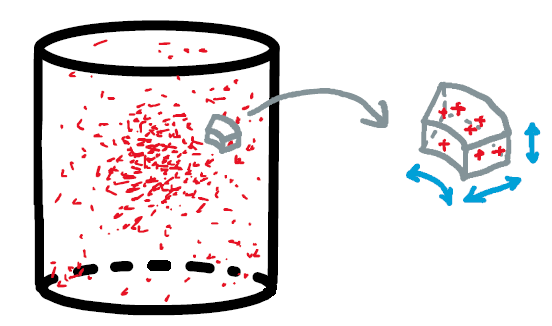
\includegraphics[width=\textwidth]{charge_vol}
\end{minipage}


Coulomb's law is then a sum of all E-field contribution from every infinitestimal charge:
\aleq{
    \vvec{E} = \inv{4\pi\epsilon_0} \frac{Q}{r^2} \hhat{r}
    \qquad\xRightarrow{\phantom{000}}\qquad
    \int \dd{\vvec{E}} 
    = \int_{\substack{\text{whole}\\\text{space}}} \inv{4\pi\epsilon_0}  \frac{\dd{Q}}{r^2}\hhat{r}
}

And the formula for electrical potential follows:
\aleq{
    V = \inv{4\pi\epsilon_0} \frac{Q}{r}
    \qquad\xRightarrow{\phantom{000}}\qquad
    \int \dd{V} 
    = \int_{\substack{\text{whole}\\\text{space}}} \inv{4\pi\epsilon_0}  \frac{\dd{Q}}{r}
}

\vskip 1em
\begin{example}
    Suppose there is a rod lying on the x-axis, 
    with its ends at $x=a$ and $x=b$.
    Let the total charge it carries be $Q$.
    What is the E-field / electric potential on an arbituary point on the z axis?
    \begin{center}
        \begin{minipage}{0.3\linewidth}
            \centering
            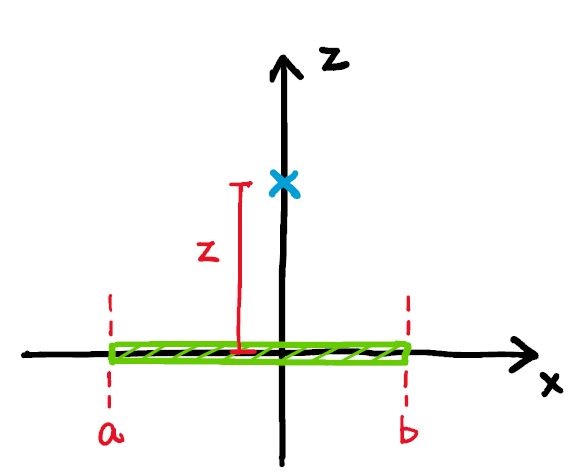
\includegraphics[width=\textwidth]{rod1}
        \end{minipage}
        \hspace{0.1\textwidth}
        \begin{minipage}{0.3\linewidth}
            \centering
            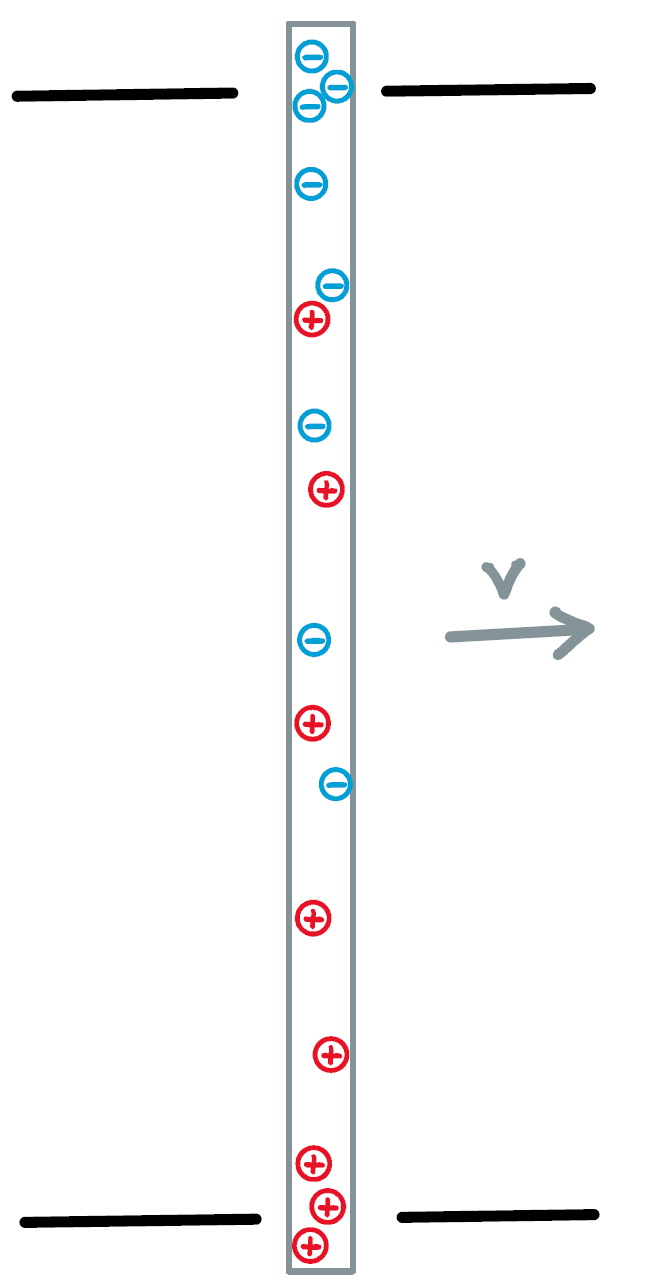
\includegraphics[width=\textwidth]{rod2}
        \end{minipage}
    \end{center}

    We can analyze by dividing the rod into infinitestimal pieces:
    \begin{itemize}
        \item Each segment has a length $\dd{x}$
        \item Charge on each segment is thus $\lambda\dd{x} = \frac{Q}{L}\dd{x}$, where $L=b-a$.
        \item For the segment at position $x$, 
        its distance from the targeted point is $\sqrt{z^2+x^2}$.
    \end{itemize}

    Thus we can calculate $V$ and $\vvec{E}$:
    \begin{enumerate}
        \item Electrical potential does not concern directions.
        So we can directly write
        \aleq{
            V = \inv{4\pi\epsilon_0}  \int_a^b \frac{\frac{Q}{L}\dd{x}}{\sqrt{z^2+x^2}}
        }

        \item Electric field concerns directions.
        So we need to resolve the direction's component from the segment to the target point. 

    \end{enumerate}
    \begin{minipage}{0.75\linewidth}
        \begin{itemize}
        \item[]
            \begin{itemize}
                \item The E-field's vertical component ($z$) should be integrated as:  
                \aleq{
                    E_z = \inv{4\pi\epsilon_0} \int_a^b \frac{\frac{Q}{L}\dd{x}}{z^2+x^2} \sin\theta 
                    = \inv{4\pi\epsilon_0}  \int_a^b \frac{\frac{Q}{L}\dd{x}}{z^2+x^2} \frac{z}{\sqrt{z^2+x^2}}
                }

                \item Similarly for the horizontal component ($x$):
                \aleq{
                    E_x = \inv{4\pi\epsilon_0} \int_a^b \frac{\frac{Q}{L}\dd{x}}{z^2+x^2}\cos\theta 
                    = \inv{4\pi\epsilon_0}  \int_a^b \frac{\frac{Q}{L}\dd{x}}{z^2+x^2} \frac{x}{\sqrt{z^2+x^2}}
                }
            \end{itemize}
        \end{itemize}
    \end{minipage}
    \hspace{0.02\textwidth}
    \begin{minipage}{0.15\linewidth}
        \centering
        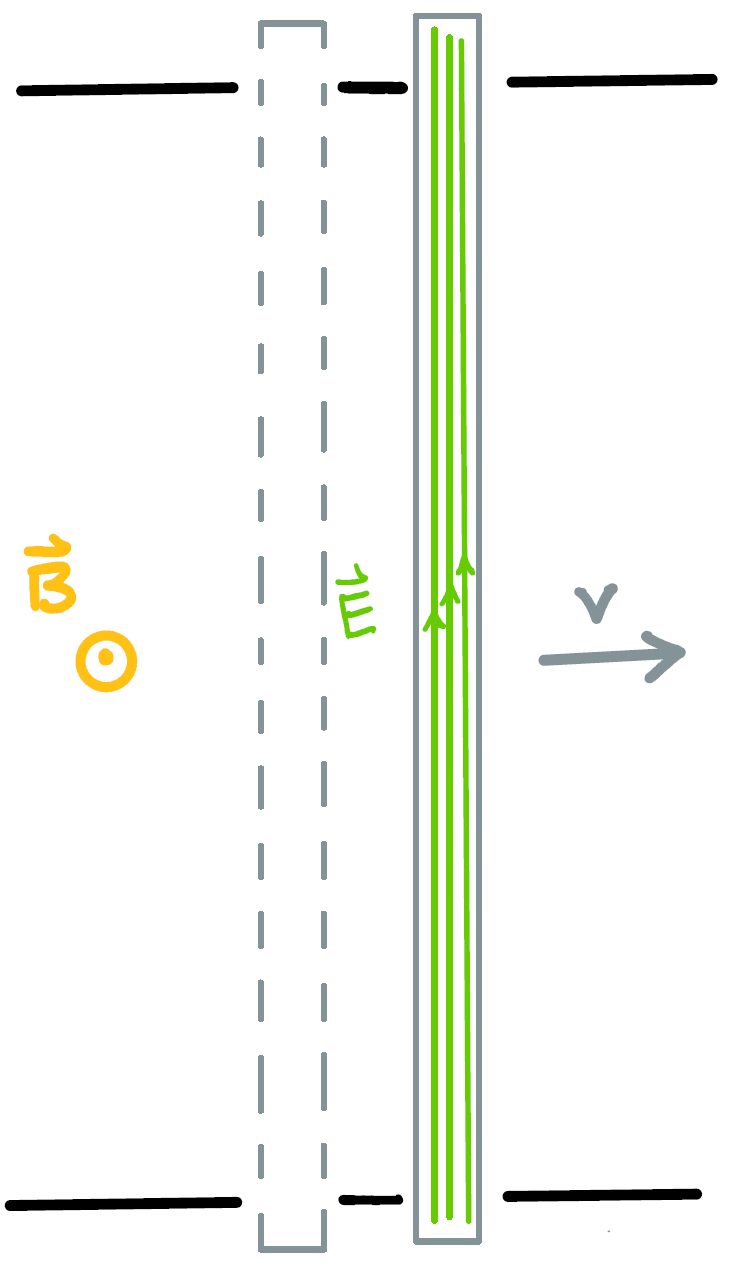
\includegraphics[width=\textwidth]{rod3}
    \end{minipage}
\end{example}

\linesep
% Section %%%%%%%%%%%%%%%%%%%%%%%%%%%%%%%%%%%%%%%%%%%%%%%%%%%%
\section{Gauss's Law}

The Gauss's Law has two different expressions:
\aleq{
    \oiint \vvec{E}\cdot \dd{\vvec{s}} &= \frac{Q}{\epsilon_0} &(\text{Integral form})\\[1ex]
    %
    \div \vvec{E} &= \frac{\rho}{\epsilon_0} &(\text{Differential form})
}

It is easier to study the physical meaning and visualize by the integral form.
After that we can generalize to the differential form by introducing an operator called \bf{divergence}.

%%%%%%%%%%%%%%
\subsection{Flux}

The literal description in Gauss's law integral form is
\aleq{
    \qty(\mstack{\text{Flux of electric field}\\\text{on a closed surface}})
    \ =\ \oiint \vvec{E}\cdot \dd{\vvec{s}}
    \ =\ \frac{Q}{\epsilon_0}
    \ =\ \frac{(\text{Charge enclosed})}{(\text{Constant})}
}
We first need to understand what \bf{flux} is, 
and what that weird integral sign even means.

%%%%%%%%%%%%%%
\subsubsection{An Analogy: A Water Pipe}

To begin with, we can make an analogy using a water pipe.
Along a normal pipe, we expect that the amount of water flowing in
should equal to the amount of water flowing out.
\begin{center}
    \begin{minipage}{0.27\linewidth}
        \centering
        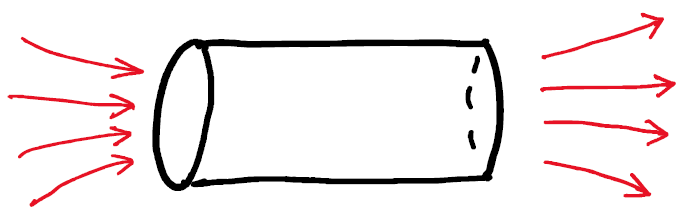
\includegraphics[width=\textwidth]{pipe}
    \end{minipage}
\end{center}

\begin{itemize}
    \item If we somehow find that the (amount of water flowing in) $>$ (amount flowing out),
    we know there is something absorbing water in the pipe!
    \begin{center}
        \begin{minipage}{0.3\linewidth}
            \centering
            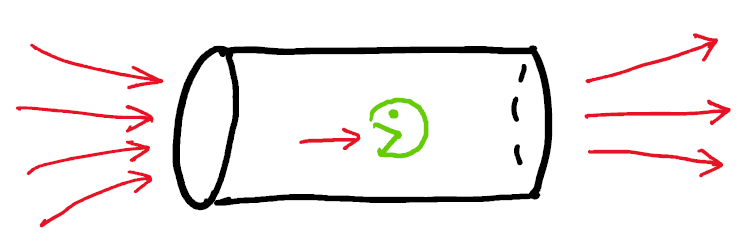
\includegraphics[width=\textwidth,trim=0 0 0 2ex]{pipe_sink}
        \end{minipage}
        \begin{minipage}{0.3\linewidth}
            \centering
            There is a "\red{sink}"\\ in the pipe!
        \end{minipage}
    \end{center}

    \item If we somehow find that the (amount of water flowing in) $<$ (amount flowing out),
    we know there is something producing water in the pipe!
    \begin{center}
        \begin{minipage}{0.3\linewidth}
            \centering
            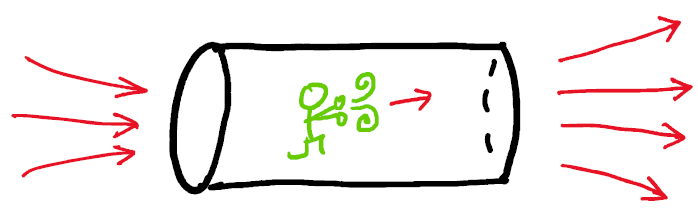
\includegraphics[width=\textwidth]{pipe_source}
        \end{minipage}
        \begin{minipage}{0.3\linewidth}
            \centering
            There is a "\red{source}"\\ in the pipe!
        \end{minipage}
    \end{center}

\end{itemize}

How can we quantitatively tell if there is a source / sink in the pipe?
We can measure by the volume flowing in / out within a short time interval $\Delta t$:
\begin{itemize}
    \item Volume flowing in = $v_\text{in}\cdot \Delta t \cdot A_\text{in} 
    = \qty(\mstack{\text{Velocity at}\\\text{entrance}})\cdot \Delta t \cdot \qty(\mstack{\text{Area of}\\\text{entrance opening}})$

    \item Volume flowing out = $v_\text{out}\cdot \Delta t \cdot A_\text{out}
     = \qty(\mstack{\text{Velocity at}\\\text{exit}})\cdot \Delta t \cdot \qty(\mstack{\text{Area of}\\\text{exit opening}})$
\end{itemize}

Then we can define a measure $\Phi = (v_\text{out}A_\text{out} - v_\text{in}A_\text{in})$
such that
\aleq{
    \begin{cases}
        \text{if }\Phi > 0 & \Rightarrow \text{ There is a source}\\
        \text{if }\Phi < 0 & \Rightarrow \text{ There is a sink}\\
    \end{cases}
}

%%%%%%%%%%%%%%
\subsubsection{Generalizing to Field}

Now use your imagination to extend idea:

\begin{enumerate}
    \item The flow of water should be continuous - 
    We can describe the flow of water by a continuous vector field $\vvec{F}(\vvec{r})$.
    \begin{center}
        \begin{minipage}{0.3\linewidth}
            \centering
            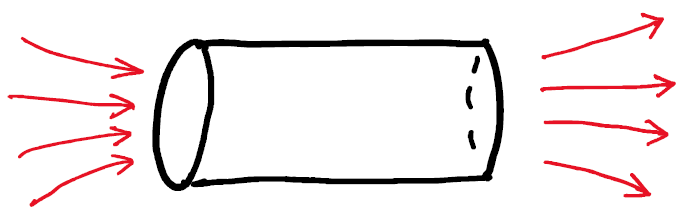
\includegraphics[width=\textwidth]{pipe}
        \end{minipage}
        \quad$\Rightarrow$\quad
        \begin{minipage}{0.3\linewidth}
            \centering
            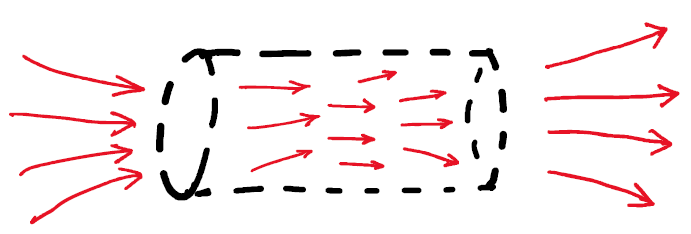
\includegraphics[width=\textwidth]{pipe_flow}
        \end{minipage}
        \quad$\Rightarrow$\quad
        \begin{minipage}{0.2\linewidth}
            \centering
            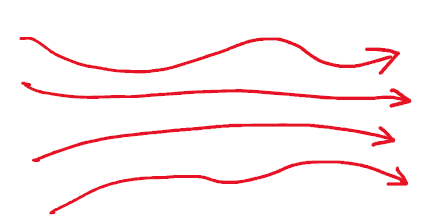
\includegraphics[width=\textwidth]{pipe_field}
        \end{minipage}
    \end{center}

    \item Our water pipe may be of any irregular shape - 
    We can "twist" the pipe into an arbituary closed surface.
    \begin{center}
        \begin{minipage}{0.16\linewidth}
            \centering
            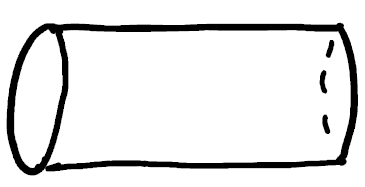
\includegraphics[width=\textwidth]{pipe_sur1}
        \end{minipage}
        \qquad$\Rightarrow$\qquad
        \begin{minipage}{0.16\linewidth}
            \centering
            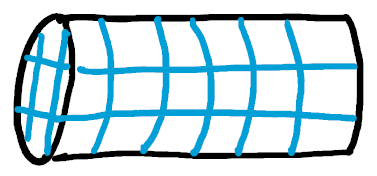
\includegraphics[width=\textwidth]{pipe_sur2}
        \end{minipage}
        \qquad$\Rightarrow$\qquad
        \begin{minipage}{0.16\linewidth}
            \centering
            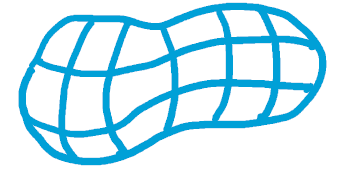
\includegraphics[width=\textwidth]{pipe_sur3}
        \end{minipage}
    \end{center}

    \ul{Note}: A "closed" surface needs to be well-distinguished between its
    "inner surface" and \phantom{\ul{Note}: } "outer surface".

\end{enumerate}

Under these circumstances,
in/out-flow are not restricted just flowing through the entrance / exit opening,
but can appear on anywhere on the surface -
each of the small grid on the surface can have a different field vector poking through it.
\begin{itemize}
    \item Out-flow = Poking from inner to outer surface
    \item In-flow = Poking from outer to inner surface
\end{itemize}

How can the flow direction be described mathematically?
We can first define a normal vector $\vvec{s}$ for each grid.
By convention, this $\vvec{s}$ 
\begin{itemize}
    \item has a magnitude equal to the surface's area of the grid.
    \item points outward of the surface (from inner to outer).
\end{itemize}

Then we can take the dot product between the field vector $\vvec{F}$ and the surface normal vector $\vvec{s}$:
\begin{itemize}
    \item If $\vvec{F}\cdot\vvec{s}>0$, 
    they are more or less in similar direction $\Rightarrow \vvec{F}$ is pointing outward!

    \item If $\vvec{F}\cdot\vvec{s}<0$,
    they are more or less in opposite direction $\Rightarrow \vvec{F}$ is pointing inward!
\end{itemize}

Finally, we define "flux" $\Phi$ over the closed surface:
\aleq{
    \Aboxed{
        \quad\Phi\quad = \sum_{\substack{\text{All small grids }i\\\text{on the closed surface}}} \vvec{F}_i \cdot \vvec{s}_i
        \quad\xrightarrow{\phantom{000}}\quad
        \tkn{oiint}{\cul[blue]{\oiint}} \vvec{F}(\vvec{r})\cdot \dd{\vvec{s}}
    }
}
\addArrow[blue]{oiint}{(0,-4ex)}
{\scriptsize A circle on double integral\\[-1ex]\scriptsize = The surface integral is over a closed surface}
{(0,-3ex)}{(0,-1ex)}

\vskip 2em
\begin{center}
    \begin{minipage}{0.9\linewidth}
        \centering
        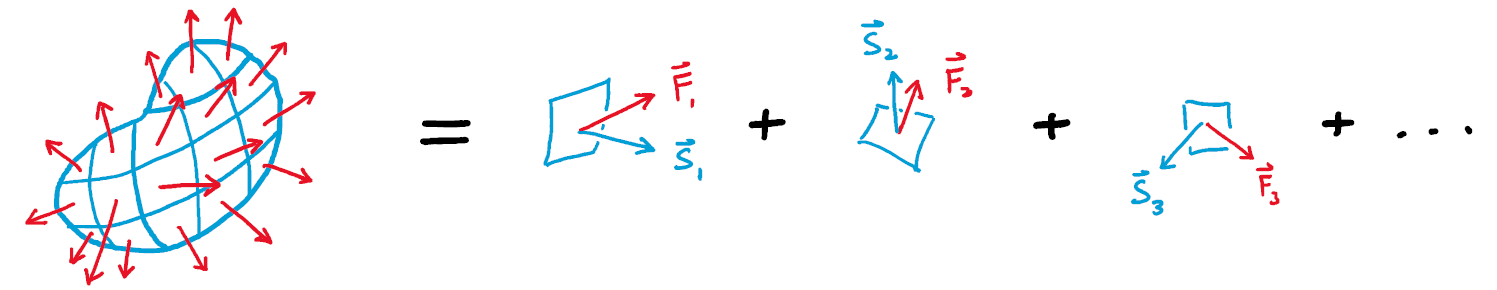
\includegraphics[width=\textwidth]{flux_int}
    \end{minipage}
\end{center}

We can use the sign of $\Phi$ to tell if there are more in-flow \gray{(or out-flow)} of field lines through the surface,
thus telling if there are sources \gray{(or sinks)} enclosed by the surface.
\begin{center}
    \begin{minipage}{0.45\linewidth}
        \centering
        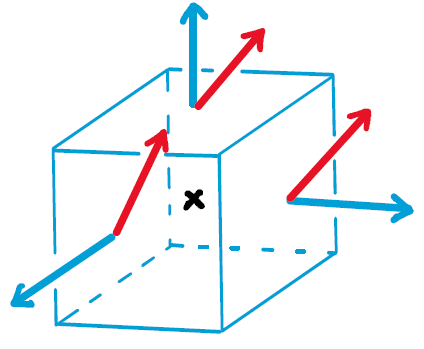
\includegraphics[width=0.7\textwidth]{flux_div}\\
        If flux $> 0$, 
        the surface likely contains\\
        \red{a diverging point} (source)
         of the field.
    \end{minipage}
    \hspace{0.01\textwidth}
    \vline
    \hspace{0.01\textwidth}
    \begin{minipage}{0.45\linewidth}
        \centering
        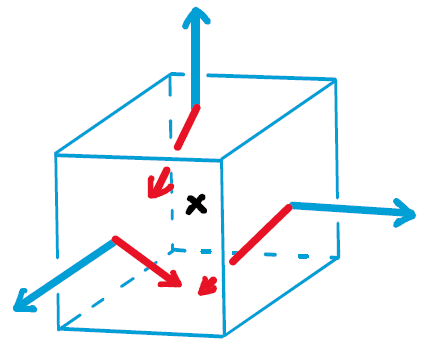
\includegraphics[width=0.7\textwidth]{flux_conv}\\
        If flux $< 0$, 
        the surface likely contains\\
        \red{a converging point} (sink)
         of the field.
    \end{minipage}
\end{center}


\vskip 1em
%%%%%%%%%%%%%%
\subsubsection{Calculation Example}

Recall that in line integral,
we have to parametrize the line before we can actually do the integral.
In calculation of flux, it is even more painful - 
it is an area integral and we have to parametrize a surface,
which is generally an impossible task without very advanced calculus.\\

Because this is just a physics course, 
here only introduces some surfaces with simple parametrization.
\bf{And in most cases we do not to calculate them when using Gauss's law.}

\begin{example}
    (Flux over a spherical surface)\\
    An easy parametrization is making use of the spherical coordinate.
    Positions on the surface can be located by the 2 anglular variables $(\theta,\phi)$:
    \aleq{
        \bmat{x\\y\\z} 
        = \bmat{x_0\\y_0\\z_0} 
        + \bmat{r\sin\theta\cos\phi\\r\sin\theta\sin\phi\\r\cos\theta} 
    }
    where $(x_0,y_0,z_0)$ indicates the center of the sphere and $r$ is the radius of the sphere.
    
    \begin{center}
        \begin{minipage}{0.2\linewidth}
            \centering
            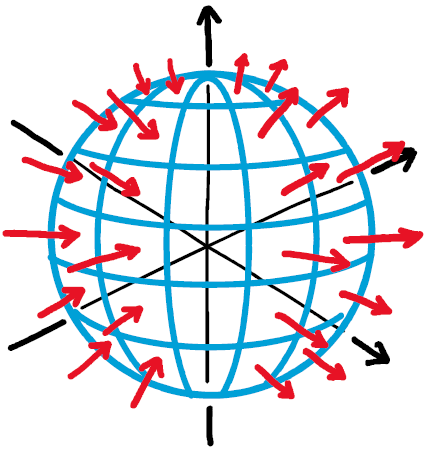
\includegraphics[width=\textwidth]{flux_sph1}
        \end{minipage}
        \hspace{0.05\textwidth}
        \begin{minipage}{0.2\linewidth}
            \centering
            with unit area as
        \end{minipage}
        \hspace{0.05\textwidth}
        \begin{minipage}{0.2\linewidth}
            \centering
            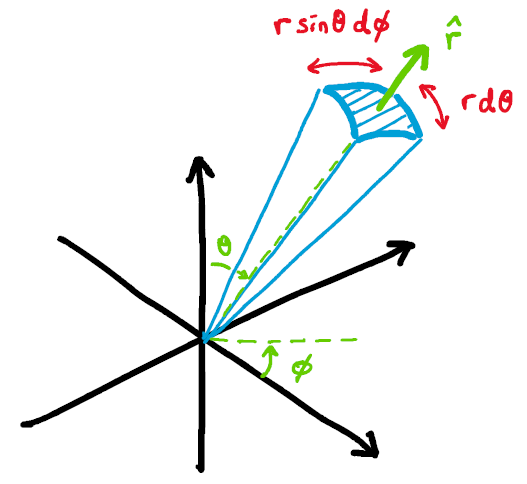
\includegraphics[width=\textwidth]{flux_sph2}
        \end{minipage}
    \end{center}
    
    The infinitestimal area is then $(r\dd{\theta})\times(r\sin\theta\dd{\phi})$
    and normal in $\hhat{r}$ direction.
    \aleq{
        \dd{\vvec{s}} = \hhat{r} r^2\sin\theta\dd{\theta}\dd{\phi}
    }

    So the flux is simply a double integral over the whole sphere surface.
    \aleq{
        \Phi = \oiint \vvec{F} \cdot \dd{\vvec{s}} 
        = \int_{\theta=0}^{\theta=\pi} \int_{\phi=0}^{\phi=2\pi} \vvec{F}(x,y,z) 
            \cdot \hhat{r} r^2\sin\theta\dd{\theta}\dd{\phi}
    }

\end{example}


\begin{example}
    (Flux over a plane)\\
    We are free to choose any two perpendicular unit vectors $\hhat{u}$,$\hhat{v}$ 
    to form a 2D coordinate system on the plane, 
    expressing a position using 2 length quantities $(u,v)$:
    \aleq{
        \bmat{x\\y\\z} 
        = \bmat{x_0\\y_0\\z_0} 
        + u\cus[blue]{\bmat{u_x\\u_y\\u_z}}{\hhat{u}} + v\cus[blue]{\bmat{v_x\\v_y\\v_z}}{\hhat{v}} 
    }
    \begin{center}
        \begin{minipage}{0.2\linewidth}
            \centering
            Choose an arbituary point 
            $(x_0,y_0,z_0)$\\ as the origin
        \end{minipage}
        \begin{minipage}{0.22\linewidth}
            \centering
            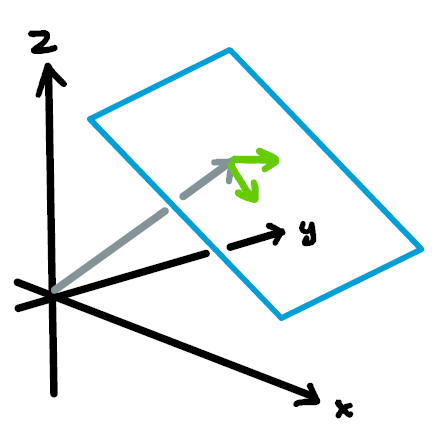
\includegraphics[width=\textwidth]{flux_plane1}
        \end{minipage}
        \qquad$\Rightarrow$\qquad
        \begin{minipage}{0.22\linewidth}
            \centering
            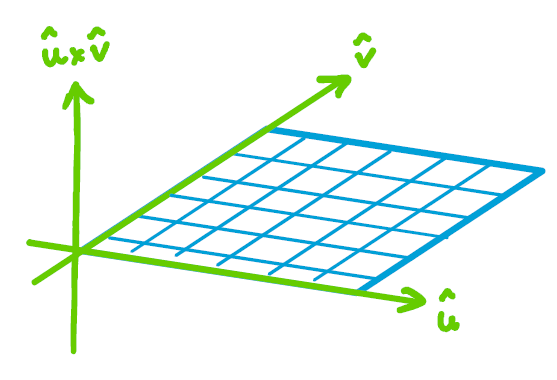
\includegraphics[width=\textwidth]{flux_plane2}
        \end{minipage}
        \begin{minipage}{0.2\linewidth}
            \centering
            Choose two arbituary directions 
            $\vvec{u},\vvec{v}$\\ as the axis
        \end{minipage}
    \end{center}

    The infinitestimal area is then $(\dd{u})\times(\dd{v})$
    and normal must be in $(\hhat{u}\cross\hhat{v})$ direction.
    \aleq{
        \dd{\vvec{s}} = (\hhat{u}\cross\hhat{v}) \dd{u}\dd{v}
    }
    So the flux is simply a double integral over a region on the plane.
    \addBentArrow[blue]{not_close}{(-5ex,-2ex)}
    {\scriptsize A plane is not a closed surface \\[-1ex]\scriptsize $\therefore$ no circle}
    {(0,-2.5ex)}{(-10ex,0)}
    \aleq{
        \Phi = \tkn{not_close}{\cul[blue]{\iint}} \vvec{F} \cdot \dd{\vvec{s}} 
        = \int_{v=c}^{v=d} \int_{u=a}^{u=b} \vvec{F}(x,y,z) 
            \cdot (\hhat{u}\cross\hhat{v})\dd{u}\dd{v}
    }
    \vskip 1em
    \begin{center}
        \begin{minipage}{0.25\linewidth}
            \centering
            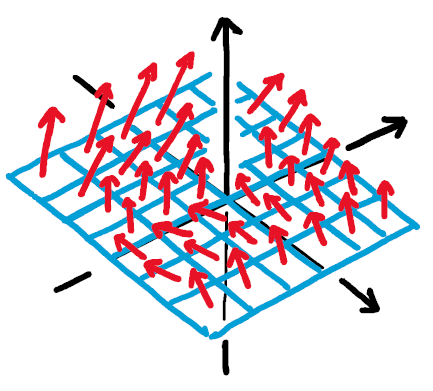
\includegraphics[width=\textwidth]{flux_plane3}
        \end{minipage}
        \hspace{0.05\textwidth}
        \begin{minipage}{0.2\linewidth}
            \centering
            with unit area as
        \end{minipage}
        \hspace{0.05\textwidth}
        \begin{minipage}{0.1\linewidth}
            \centering
            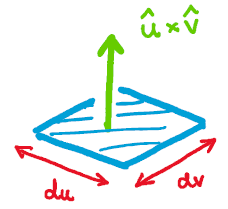
\includegraphics[width=\textwidth]{flux_plane4}
        \end{minipage}
    \end{center}

\end{example}

\vskip 1ex
%%%%%%%%%%%%%%
\subsection{Divergence}

However there is a problem in using flux - 
if we choose the surface too arbituarily, 
the calculated flux is no longer meaningful.
\begin{center}
    \begin{minipage}{0.35\linewidth}
        \centering
        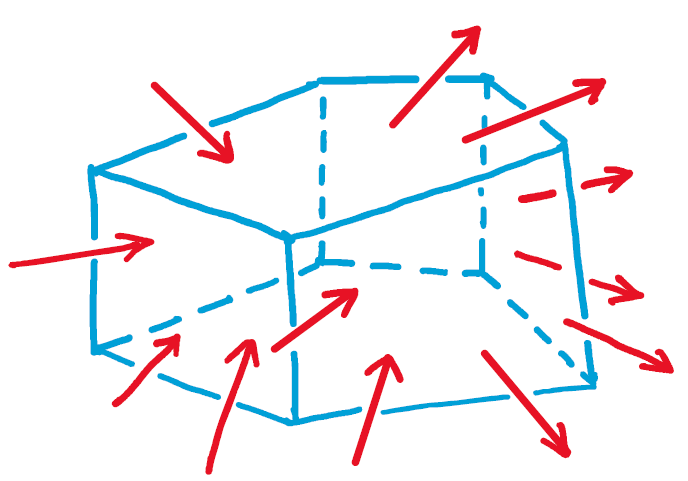
\includegraphics[width=\textwidth]{flux_mess}
    \end{minipage}
    \hspace{0.05\textwidth}
    \begin{minipage}{0.45\linewidth}
        \centering
        E.g. If we choose a very big surface and calculate the flux $\approx 0$, 
        Does it tells us where the diverging/converging points are?
    \end{minipage}
\end{center}


To tackle this problem,
we need to introduce the \bf{divergence} operator:
\aleq{
    \tkn{div}{\cul[red]{\div}}\ \bullet
    \ \defeq\ \divRec{\bullet}
    \ \defeq\ \tkn{div2}{\cul[blue]{\text{div}}}\ \bullet
}
\addArrow[red]{div}{(0,-3ex)}
{\scriptsize Like gradient operator\\[-1ex]\scriptsize but with a dot}
{(0,-1ex)}{(0,-1ex)}
\addArrow[blue]{div2}{(0,-3ex)}
{\scriptsize Sometimes we\\[-1ex]\scriptsize just write "div"}
{(0,-1ex)}{(0,-1ex)}


\vskip 1em
The divergence operator can be applied on a vector function,
and it returns a scalar (number) function.
\aleq{
    \div \vvec{F} 
    &= \bmat{\pdvv{x} & \pdvv{y} & \pdvv{z}}\bmat{F_x\\F_y\\F_z}\\[1ex]
    &= \pdvv{F_x}{x} + \pdvv{F_y}{y} + \pdvv{F_z}{z}\\[1ex]
    &= (\text{A number})
}

The divergence of a vector field is related to its
\bf{total flux through an infinitestimally small but closed surface.}

%%%%%%%%%%%%%%
\subsubsection{Geometrical Interpretation}

To visualize, we can draw an infinitestimal small cube around a point $(x,y,z)$.
Although a cube has 6 faces, 
because of symmetry in all 3 directions,
it suffices to just analyze by the 2 faces that are parallel to the $x$-$y$ plane.
\begin{center}
    \begin{minipage}{0.3\linewidth}
        \centering
        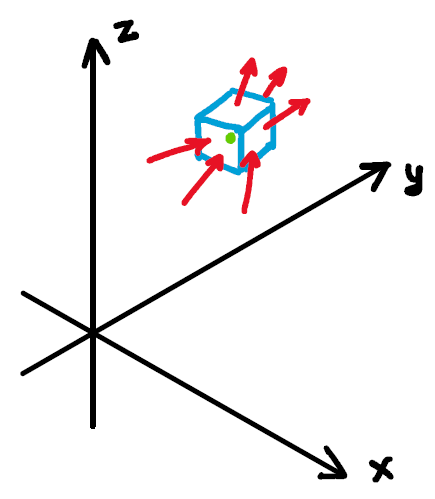
\includegraphics[width=0.7\textwidth]{flux_elem1}
    \end{minipage}
    \qquad{\huge $\Rightarrow$}\qquad\ 
    \begin{minipage}{0.5\linewidth}
        \centering
        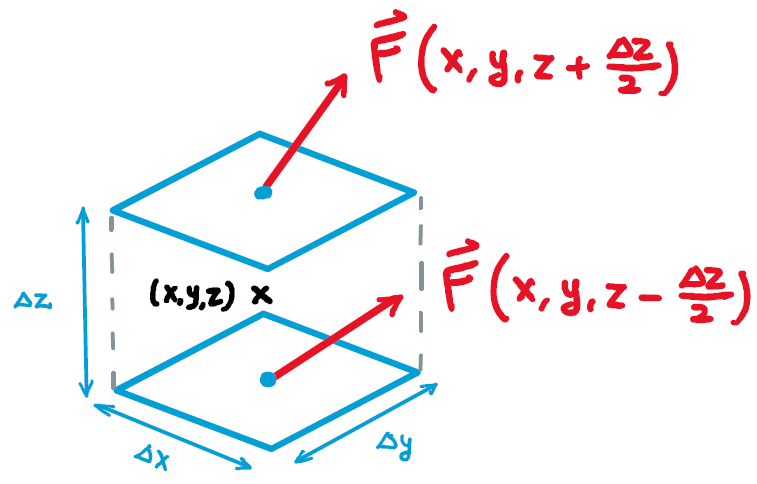
\includegraphics[width=\textwidth]{flux_elem2}
    \end{minipage}
\end{center}

\vskip 1ex
\begin{itemize}
    \item Normal direction of these 2 faces = $\hhat{z}$ \ $\Rightarrow$\ 
    The surface normal vector $=\blue{(\Delta x \Delta y) \hhat{z}}$.

    \item Center point of top surface = $\qty(x,y,z+\frac{\Delta z}{2})$ 
    \ $\Rightarrow$\ The field pokes through it $=\red{\vvec{F}\qty(x,y,z+\frac{\Delta z}{2})}$.

    \item Center point of bottom surface = $\qty(x,y,z-\frac{\Delta z}{2})$ 
    \ $\Rightarrow$\ The field pokes through it $=\red{\vvec{F}\qty(x,y,z-\frac{\Delta z}{2})}$.

\end{itemize}

Therefore the total flux through the 2 planes is
\aleq{
    \qty(\mstack{\text{Total Out-flux through}\\[0.5ex]\text{surfaces}\sparallel\text{x-y plane}}) 
    &= \qty(\mstack{\text{Out-flux through}\\[0.5ex]\text{top face}}) - 
        \qty(\mstack{\text{In-flux through}\\[0.5ex]\text{bottom face}})\\[1em]
    %
    \dd{\Phi_{xy}} &= 
    \textstyle \vvec{F}\qty(x,y,z+\frac{\Delta z}{2}) \cdot \hhat{z} (\Delta x \Delta y) - 
        \vvec{F}\qty(x,y,z-\frac{\Delta z}{2}) \cdot \hhat{z} (\Delta x \Delta y)\\[1em]
    %
    &= \qty(\frac{\vvec{F}\qty(x,y,z+\frac{\Delta z}{2}) - \vvec{F}\qty(x,y,z-\frac{\Delta z}{2})}{\blue{\Delta z}}) 
        \cdot \hhat{z} (\Delta x \Delta y\blue{\Delta z})\\[1ex]
    %
    &= \cut[red]{\cbox[red]{\qty(\frac{\vvec{F}\qty(x,y,\cbox[red]{\textstyle z+\frac{\Delta z}{2}}) 
        - \vvec{F}\qty(x,y,\cbox[red]{\textstyle z-\frac{\Delta z}{2}})}{\cbox[red]{\Delta z}})}}{\text{This is exactly partial z}}
        \cdot \hhat{z} (\Delta x \Delta y \Delta z)\\[1ex]
    %
    &= \pdvv{z}\cul[green]{\vvec{F}(x,y,z)\cdot \hhat{z}} (\Delta x \Delta y\Delta z)\\[1em]
    %
    &= \pdvv{z}\tkn{div_dot}{\cul[green]{F_z}}(x,y,z)\ (\Delta x \Delta y\Delta z)\\[1em]
    %
    &= \qty(\mstack{\text{Divergence's }\\[0.5ex] z\text{ term}})\ \qty(\mstack{\text{Unit}\\[0.5ex]\text{volume}})
}
\addArrow[green]{div_dot}{(3ex,6ex)}{\scriptsize Dot product to $\hhat{z}$ = Only take $z$ component}{(0,2ex)}{(15ex,-3.5ex)}

We can expect the similar results in the other 2 directions.
Gather them together:
\aleq{
    \qty(\mstack{\text{Total flux through}\\[0.5ex]\text{the volume}})
    %
    &=\qty(\mstack{\text{Total flux through}\\[0.5ex]\text{surfaces}\sparallel\text{y-z plane}})
    + \qty(\mstack{\text{Total flux through}\\[0.5ex]\text{surfaces}\sparallel\text{x-z plane}}) 
    + \qty(\mstack{\text{Total flux through}\\[0.5ex]\text{surfaces}\sparallel\text{x-y plane}})\\[1ex]
    %
    &= \qty[\qty(\mstack{\text{Divergence's }\\[0.5ex] x\text{ term}})
    + \qty(\mstack{\text{Divergence's }\\[0.5ex] y\text{ term}})
    + \qty(\mstack{\text{Divergence's }\\[0.5ex] z\text{ term}})]
    \ \qty(\mstack{\text{Unit}\\[0.5ex]\text{volume}})\\[1ex]
    %
    \dd{\Phi} &= \qty[\pdvv{F_x}{x} + \pdvv{F_y}{y} + \pdvv{F_z}{z}](\dd{x}\dd{y}\dd{z})\\[1ex]
    %
    &= \qty(\div \vvec{F})(\dd{x}\dd{y}\dd{z})
}

\vskip 1ex
Therefore we can geometrically interpret divergence as
\aleq{
    \Aboxed{
        \qty(\text{\bf{Divergence}}) 
        = \div \vvec{F} 
        \sim \frac{\dd{\Phi}}{\dd{x}\dd{y}\dd{z}} 
        = \frac{(\text{Flux through a closed surface})}{(\text{Volume enclosed by the surface})}
        \sim (\text{\bf{Flux \tkn{flux_density}{\cul[blue]{density}}}})
    }
}
\addArrow[blue]{flux_density}{(0,-4ex)}{\scriptsize This density\\[-1ex]\scriptsize is by volume}{(0,-1ex)}{(0,-1ex)}

\vskip 1em
%%%%%%%%%%%%%%
\subsubsection{Divergence Theorem}

With the geometrical interpretation,
we can directly state (without proof) a convenient formula related to divergence - 
the \bf{divergence theorem}:
\aleq{
    \Aboxed{
        \oiint \vvec{F}\cdot \dd{\vvec{s}} &= \iiint (\div \vvec{F}) \dd{\tau}
    }
}

which can be literally interpret as
\aleq{
    \qty(\mstack{\text{Total }\\[0.5ex]\text{Flux}})
    \quad \sim \sum_{\text{All volumes}} \qty(\mstack{\text{Flux}\\[0.5ex]\text{per volume}})\times \qty(\text{Volume})
}


%%%%%%%%%%%%%%
\subsection{Gauss's Law - Explanation}


The Gauss's law is purely an \cul[red]{observation} about the relation between E-field and charges:
\aleq{
    \Aboxed{
        \mstack{\text{Total flux of E-field on }\\[0.5ex]\text{a closed surface}\neq 0}
        \qquad\Leftrightarrow\qquad
        \mstack{\text{There are charges}\\[0.5ex]\text{inside the surface}}
    }
}

The two forms of Gauss's law are describing this same observation:
\begin{itemize}
    \item \ul{Integral form}:
    \vskip -5ex
    \aleq{
        (\vvec{E}\text{'s flux})\ \sim\ \oiint \vvec{E}\cdot\dd{\vvec{s}} 
        \ =\ \frac{Q}{\epsilon_0} \ \sim\ (\text{Charge})
    }

    \item \ul{Differential form}:
    \vskip -5ex
    \aleq{
        \qty(\mstack{\vvec{E} \text{'s flux}\\[0.5ex]\text{density}})\ \sim\ \div \vvec{E}
        \ =\ \frac{\rho}{\epsilon_0} \ \sim\ \qty(\mstack{\text{Charge}\\[0.5ex]\text{density}})
    }
\end{itemize}

And the two form can be inter-converted by divergence theorem.
\addArrow[red]{divE}{(0,9ex)}{Divergence Theorem}{(1ex,3ex)}{(-12ex,-6ex)}
\addBentArrow[blue]{divQ}{(-4ex,13ex)}{Charge to Charge density}{(1ex,3ex)}{(18ex,-8ex)}
\aleq{
    \oiint \vvec{E}\cdot\dd{\vvec{s}} \quad &=\quad \frac{Q}{\epsilon_0}\\[2em]
    \tkn{divE}{\iiint (\div \vvec{E}) \dd{\tau}}\ &=\ \inv{\epsilon_0}\tkn{divQ}{\iiint \rho \dd{\tau}}
}



%%%%%%%%%%%%%%
\subsection{Applying Gauss's Law Integral Form}

In beginner electromagnetism, 
there is only one type of problem related to Gauss's law : 
\quoting{
    Given the charge distribution, 
    find the E-field everywhere by Gauss's law integral form\\
    in some \cul[red]{very symmetrical} scenarios.
}
which is basically asking you to \it{revert} the flux calculation:
\aleq{
    \oiint \vvec{E}\cdot\dd{\vvec{s}} = \frac{Q}{\epsilon_0}
    \qquad\Rightarrow\qquad
    \vvec{E} = \text{Some function of }Q
}

If $Q$ has a very ugly distribution, 
there is nothing we can do other than solving some PDEs.
But \red{if $Q$ distributes very symmetrically, 
$\vvec{E}$ should also be symmetrical}, 
such that the flux integral can be broken into multiplications.\\

In these cases, we can choose a "Gaussian" surface to to be integrated where
\begin{enumerate}
    \item $\vvec{E}$ has constant magnitude everywhere on the surface.
    \item $\vvec{E}$ forms the same angle with the surface normal vector everywhere on the surface
\end{enumerate}

\vskip 1ex
Only then, the flux integral can be broken down as
\aleq{
    \oiint \vvec{E}\cdot \dd{\vvec{s}} 
    &= \oiint \tkn{gauss_dot}{\cul[green]{\norm{\vvec{E}}\norm{\dd{\vvec{s}}}\cos\theta}}\\[1ex]
    &= \tkn{gauss_E}{\cul[red]{\norm{\vvec{E}}}}\ \tkn{gauss_theta}{\cul[blue]{\cos\theta}}\ \oiint \norm{\dd{\vvec{s}}}\\[2.5em]
    &= \norm{\vvec{E}}\ \cos\theta\ (\text{Total surface area})
}
\addArrow[green]{gauss_dot}{(5ex,0)}
{\scriptsize Just dot product\\[-1ex]\scriptsize $\vvec{a}\cdot\vvec{b}=\norm{\vvec{a}}\norm{\vvec{b}}\cos\theta$}
{(8ex,0)}{(6ex,0)}
\addBentArrow[red]{gauss_E}{(-8ex,-3.5ex)}
{Same magnitude everywhere\\[-0.5ex]Can move out of integral!}
{(0,-1.5ex)}{(-12.5ex,1ex)}
\addBentArrow[blue]{gauss_theta}{(8ex,-3.5ex)}
{Form same angle everywhere\\[-0.5ex]Can move out of integral!}
{(0,-1.5ex)}{(12.5ex,1ex)}

such that we can find the magnitude of $\vvec{E}$ with simple division
\aleq{
    \Aboxed{
        \norm{\vvec{E}} 
        = \frac{(\text{Total flux})}{(\text{Total surface area})\cos\theta}
        = \frac{Q/\epsilon_0}{(\text{Total surface area})\cos\theta}
    }
}

In fact, there are not many of these "very symmetrical" cases.
These examples below, with their respective Gaussian surfaces,
are basically all the variations you can find in textbooks.

\begin{center}
    \begin{tabular}{>{\centering\arraybackslash}m{0.3\linewidth}
        >{\centering\arraybackslash}m{0.3\linewidth}
        >{\centering\arraybackslash}m{0.3\linewidth}}
        \makecell{Charge configuration\\(Assuming uniform density)} 
        & & Good Gaussian surface 
        \\[1ex]
        \hline
        Sphere
        &
        \vskip 1ex
        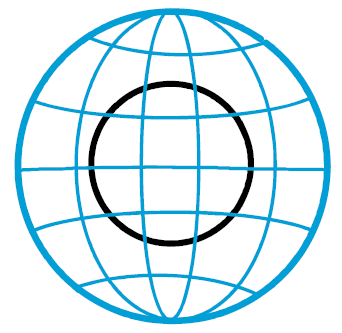
\includegraphics[width=0.55\linewidth]{sph_out}
        &
        \blue{Spherical shell}
        \\[1ex]
        %
        Infinitely long rod / cylinder
        &
        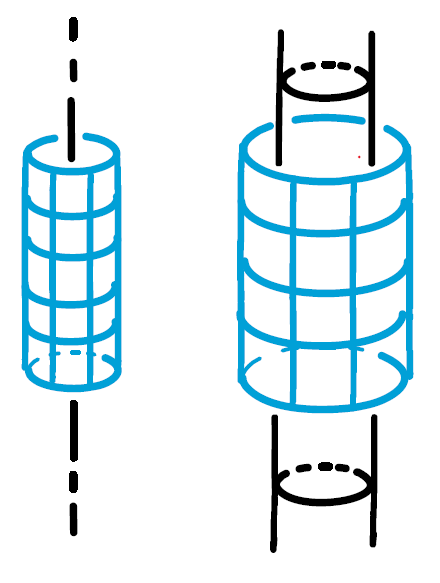
\includegraphics[width=0.6\linewidth]{cyl}
        &
        \blue{Curved face of cylinder}
        \\[1ex]
        %
        Infinitely large plane
        &
        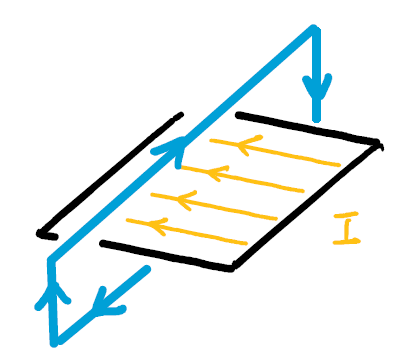
\includegraphics[width=0.9\linewidth]{plane}
        &
        \blue{Infinitely large planes wrapping it around}
        \\[3em]
        %
        Finite long rod 
        &
        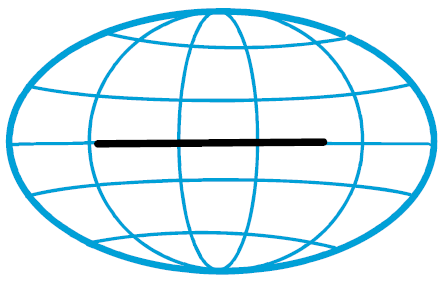
\includegraphics[width=0.7\linewidth]{ellipse}
        &
        \blue{\makecell{Ellipsoid with foci\\ = end points of the rod}}
        \\
        \hline
    \end{tabular}
\end{center}

\vskip 1ex
\ul{P.S.} In electrostatics (no moving charges), 
all good Gaussian surfaces are equipotential surfaces.


\begin{example}
    Given a solid sphere with uniform charge density $\rho$ and radius $R$.
    By spherical symmetry, the E-field must satisfy:

    \begin{minipage}{0.7\linewidth}
        \begin{itemize}
            \item Only point in radial direction.
            \item Magnitude does not depend on angular directions $\theta,\phi$.
        \end{itemize}
    \end{minipage}
    \begin{minipage}{0.15\linewidth}
        \centering
        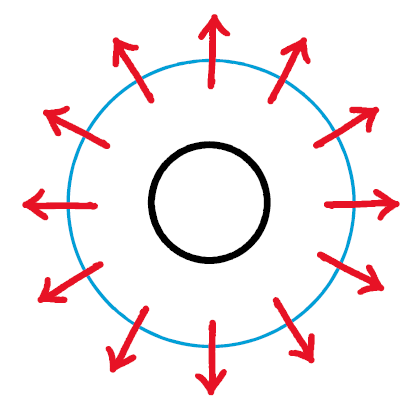
\includegraphics[width=\textwidth]{sph_sym}
    \end{minipage}

    \vskip 1em
    Therefore we can choose the Gaussian surface to be a sphere of radius $r$ 
    to find the magnitude of E-field at distance $r$ from the sphere center.
    \addArrow[green]{gauss_sphth}{(7ex,0)}
    {\scriptsize E-field = radial \\[-1ex]\scriptsize $\therefore$ Normal to surface}{(2ex,0.5ex)}{(5.5ex,1ex)}
    \addArrow[blue]{gauss_sphr}{(3ex,0)}
    {\scriptsize You have to manually add the unit vector}{(2ex,0.5ex)}{(15ex,0)}
    \aleq{
        \norm{\vvec{E}} 
        &= \frac{Q/\epsilon_0}{(\text{Total surface area})\cos\theta}\\
        &= \frac{Q}{\epsilon_0} \cdot \inv{(4\pi r^2)} \cdot \inv{\cos \tkn{gauss_sphth}{\cul[green]{0^\circ}}}\\
        &= \frac{Q}{4\pi\epsilon_0 r^2}\\[1ex]
        \Rightarrow\quad \vvec{E} &= \frac{Q}{4\pi\epsilon_0 r^2} \tkn{gauss_sphr}{\cul[blue]{\hhat{r}}}
    }
    
    \begin{enumerate}
        \item For radial distance $r < R$,
        the total charge enclosed in the gaussian surface is only the core of the sphere,
        up to radius $r$. So we should take $Q=\frac{4}{3}\pi r^3\rho$.
        \begin{center}
            \begin{minipage}{0.4\linewidth}
                \aleq{
                    \vvec{E} 
                    &= \frac{\qty(\frac{4}{3}\pi r^3 \rho)}{4\pi\epsilon_0 r^2}\hhat{r} 
                    = \frac{\rho r}{3\epsilon_0} \hhat{r}
                }
            \end{minipage}
            \hspace{0.05\textwidth}
            \begin{minipage}{0.15\linewidth}
                \centering
                
\includegraphics[width=\textwidth]{sph_in}
            \end{minipage}
        \end{center}

        \item For radial distance $r > R$
        the total charge enclosed in the gaussian surface is the whole sphere,
        So we should take $Q=\frac{4}{3}\pi R^3\rho$.
        \begin{center}
            \begin{minipage}{0.4\linewidth}
                \aleq{
                    \vvec{E}
                    &= \frac{\qty(\frac{4}{3}\pi R^3 \rho)}{4\pi\epsilon_0 r^2}\hhat{r} 
                    = \frac{\rho R^3}{3\epsilon_0 r^2} \hhat{r}
                }
            \end{minipage}
            \hspace{0.05\textwidth}
            \begin{minipage}{0.15\linewidth}
                \centering
                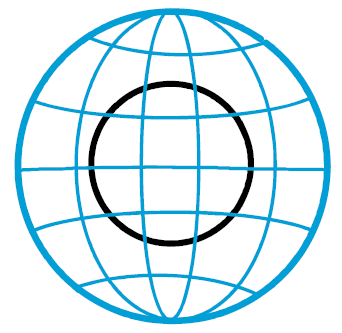
\includegraphics[width=\textwidth]{sph_out}
            \end{minipage}
        \end{center}

    \end{enumerate}
    
\end{example}

\vskip 2em
\begin{example}
    Given an infinitely long hollow cylinder with inner radius $=a$ and outer radius $=b$,
    and its charge density is proportional to distance from center $r$, i.e. $\rho(\vvec{r}) =kr$.\\
    
    For cylinder, we can claim by cylindrical symmetry 
    that the E-field must satisfy:

    \begin{minipage}{0.55\linewidth}
        \begin{itemize}
            \item Only point in $r$ direction.
            \item Magnitude does not depend on $\theta$ or $z$.
        \end{itemize}
    \end{minipage}
    \begin{minipage}{0.1\linewidth}
        \centering
        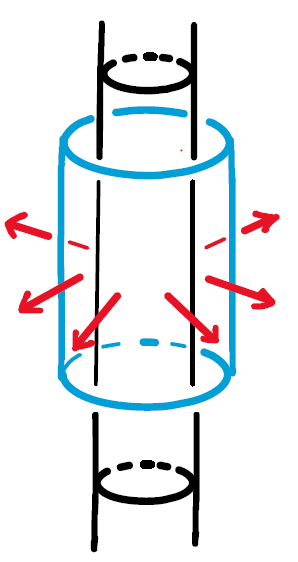
\includegraphics[width=\textwidth]{cyl_sym}
    \end{minipage}

    Therefore we can choose the Gaussian surface to be a cylindrical sheet radius $r$ 
    and an arbituary length $L$ (which will be cancelled later)
    to find the magnitude of E-field at distance $r$ from the rotation axis.
    \aleq{
        \norm{\vvec{E}} 
        &= \frac{Q/\epsilon_0}{(\text{Total surface area})\cos\theta}\\
        &= \frac{Q}{\epsilon_0} \cdot \tkn{gauss_cylcurve}{\cul[red]{\inv{(2\pi r L)}}} \cdot \inv{\cos \tkn{gauss_cylth}{\cul[green]{0^\circ}}}\\[1em]
        &= \frac{Q}{2\pi\epsilon_0 r L}\\[1ex]
        \Rightarrow\quad \vvec{E} &= \frac{Q}{2\pi\epsilon_0 r L} \tkn{gauss_cylr}{\cul[blue]{\hhat{r}}}
    }
    \addBentArrow[red]{gauss_cylcurve}{(7ex,-4ex)}
    {\scriptsize E-field = radial \\[-1ex]\scriptsize $\therefore$ Only go through the curved surface \\[-1ex]\scriptsize Top/bottom surface has no flux}
    {(0,-3ex)}{(12ex,1ex)}
    \addArrow[green]{gauss_cylth}{(7ex,0)}
    {\scriptsize E-field = radial \\[-1ex]\scriptsize $\therefore$ Normal to curved surface}{(2ex,0.5ex)}{(8.5ex,1ex)}
    \addArrow[blue]{gauss_cylr}{(3ex,0)}
    {\scriptsize You have to manually add the unit vector}{(2ex,0.5ex)}{(15ex,0)}

    This time the charge density depends on position,
    so the total charge enclosed by the surface needs to be computed by integration.

    \begin{minipage}{0.7\linewidth}
        \begin{enumerate}
            \item For radial distance $r<a$, there is no charge enclosed because the cylinder is hollow.
            So $Q=0$ implying $\vvec{E}=0$.
        \end{enumerate}
    \end{minipage}
    \hspace{0.05\textwidth}
    \begin{minipage}{0.2\linewidth}
        \centering
        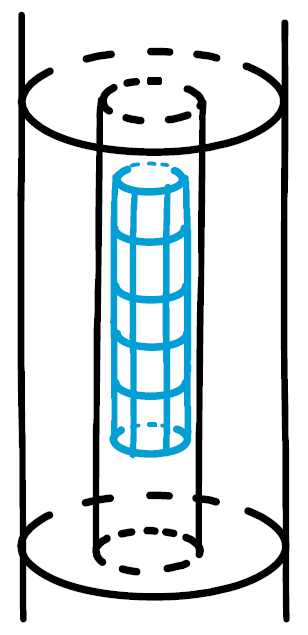
\includegraphics[height=10em]{cyl_in}
    \end{minipage}

    \vskip 2em
    \begin{minipage}{0.7\linewidth}
        \begin{enumerate}
            \item[2.] For radial distance $a<r<b$, 
            total enclosed charge are distributed from radius $=a$ to radius $=r$,
            which calculates as
            \aleq{
                Q = \int^r_a \rho \cdot 2\pi rL\dd{r} 
                =  2\pi kL \int^r_a r^2 \dd{r} 
                =  \frac{2\pi kL}{3} (r^3-a^3)
            }
            So the E-field is
            \aleq{
                \vvec{E} = \frac{Q}{2\pi\epsilon_0 r L}\hhat{r} 
                = \frac{k}{3\epsilon_0}\qty(r^2 - \frac{a^3}{r}) \hhat{r}
            }
        \end{enumerate}
    \end{minipage}
    \hspace{0.05\textwidth}
    \begin{minipage}{0.2\linewidth}
        \centering
        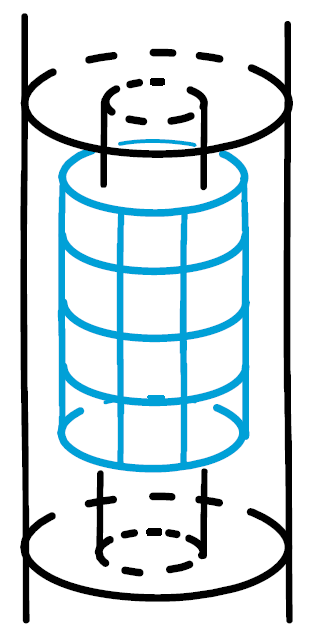
\includegraphics[height=10em]{cyl_mid}
    \end{minipage}

    \vskip 2em
    \begin{minipage}{0.7\linewidth}
        \begin{enumerate}
            \item[3.] For radial distance $r>b$,
            total enclosed charge are distributed from radius $=a$ to radius $=b$,
            which calculates as
            \aleq{
                Q = \int^b_a \rho \cdot 2\pi rL\dd{r} 
                =  2\pi kL \int^r_a r^2 \dd{r} 
                =  \frac{2\pi kL}{3} (b^3-a^3)
            }
            So the E-field is
            \aleq{
                \vvec{E} = \frac{Q}{2\pi\epsilon_0 r L}\hhat{r} 
                = \frac{k}{3\epsilon_0r}\qty(b^3 - a^3) \hhat{r}
            }
        \end{enumerate}
    \end{minipage}
    \hspace{0.05\textwidth}
    \begin{minipage}{0.2\linewidth}
        \centering
        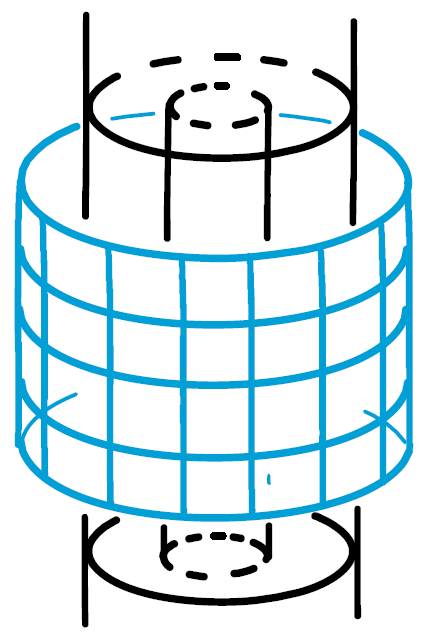
\includegraphics[height=10em]{cyl_out}
    \end{minipage}

\end{example}



\linesep
% Section %%%%%%%%%%%%%%%%%%%%%%%%%%%%%%%%%%%%%%%%%%%%%%%%%%%%
\section{Electric Potential}

%%%%%%%%%%%%%%
\subsection{Mathematical Origin}

The reason to create a electrical potential function $V(\vvec{r})$ is rather mathematical:
\begin{itemize}
    \item \ul{Observation}: 
    E-field by static charge never forms loops.
    $\Rightarrow$ Static E-field is conservative.

    \item \ul{Mathematical fact}: 
    Any conservative field can be expressed as the gradient of some scalar function (i.e. potential).
\end{itemize}

Therefore we can define a scalar function $V(\vvec{r})$ such that 
\aleq{
    \Aboxed{
        \vvec{E}(\vvec{r}) = - \grad V(\vvec{r})
    }
}

And the reverse can be calculated by 
\aleq{
    \Aboxed{
        V(\vvec{r_0}) 
        = -\int_{\substack{\text{any path}\\\text{from }\infty\text{ to }\vvec{r_0}}} \vvec{E}(\vvec{r}) \cdot \dd{\vvec{r}}
        = -\int_\infty^{\vvec{r_0}} \vvec{E}(\vvec{r})\dd{\vvec{r}}
    }
}

%%%%%%%%%%%%%%
\subsection{Poisson Equation}

If we substitute $\vvec{E} = -\grad V$ into the Gauss's law,
we arrive at a new equation: 
\addBelowArrow[blue]{laplacian1}{laplacian2}{\scriptsize This is called\\[-1ex]\scriptsize \bf{Laplacian Operator}}{-1ex}{(0,-2ex)}
\aleq{
    \frac{\rho}{\epsilon_0} &= \div \vvec{E}\\
    &= \div (-\grad V)\\
    &= - \div \qty(\pdvv{V}{x}\hhat{x} + \pdvv{V}{y}\hhat{y} + \pdvv{V}{z}\hhat{z})\\
    &= - \qty(\tkn{laplacian1}{\cul[blue]{\pdvv[2]{V}{x} + \pdvv[2]{V}{y} + \pdvv[2]{V}{z}}}) 
    \defeq \ -\tkn{laplacian2}{\cul[blue]{\laplacian}} V\\[2em]
    \Aboxed{
        \laplacian V(\vvec{r}) &= -\frac{\rho(\vvec{r})}{\epsilon_0}
    }
}

\vskip 1ex
This equation belongs to a class of PDE called \bf{Poisson equation}, 
which is one of the earliest studied PDEs in history.
It is \cul[red]{the most fundamental relation between potential and charge}.
Given any configurations of charge or potential,
idealy we can find the other using this PDE.
\begin{itemize}
    \item \ul{$V(\vvec{r})$ to $\rho(\vvec{r})$} : 
    Computing $\laplacian$ is just a sum of \nth{2} order derivatives. (Easy!)

    \item \ul{$\rho(\vvec{r})$ to $V(\vvec{r})$} : 
    Need to solve the Laplacian equation,
    which is a \nth{2} order non-homogeneous
    \\ \phantom{\ul{$\rho(\vvec{r})$ to $V(\vvec{r})$} :} linear PDE. (Awful!)
\end{itemize} 

Unfortunately in realistic problems,
it is more frequent to ask for $V(\vvec{r})$ (or $\vvec{E}(\vvec{r})$) from $\rho(\vvec{r})$,
because we can usually confine the charge distribution in a small region by using very small test objects;
but for potential and E-field, they are always everywhere. 
\begin{center}
    \begin{minipage}{0.15\linewidth}
        \centering
        {\small It is easy to make $\rho=0$\\ in most places}
    \end{minipage}
    \begin{minipage}{0.27\linewidth}
        \centering
        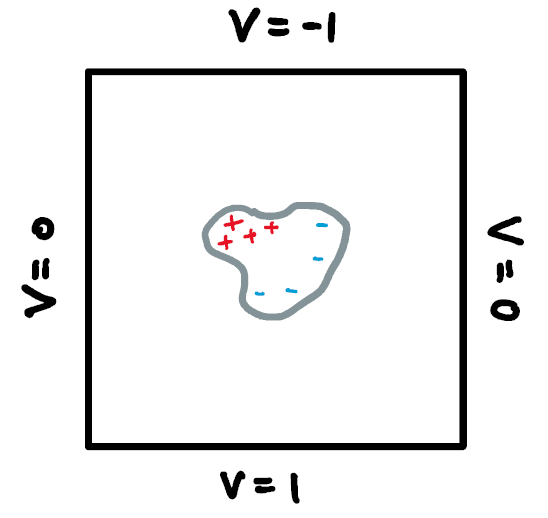
\includegraphics[width=\textwidth]{poisson_Q}
    \end{minipage}
    {\Large \quad$\Leftrightarrow$\quad}
    \begin{minipage}{0.27\linewidth}
        \centering
        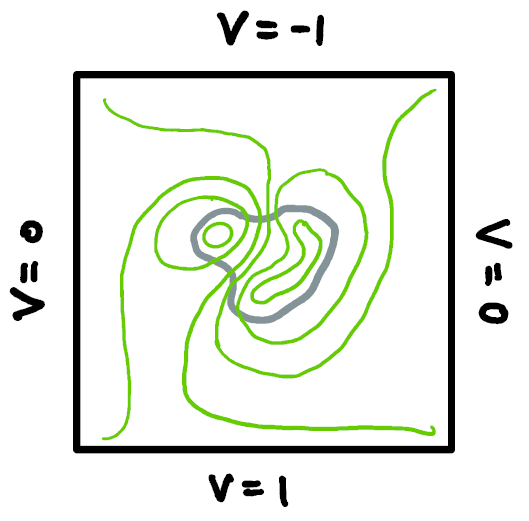
\includegraphics[width=\textwidth]{poisson_V}
    \end{minipage}
    \begin{minipage}{0.15\linewidth}
        \centering
        {\small It is difficult\\ to know $V$ everywhere}
    \end{minipage}
\end{center}

We are not going to discuss how to solve the Poisson equation here - 
it can take several book chapters to analyze the solution forms at different boundary conditions.
(And in many cases, we need to resort to numerical methods.)
Those shall be left to the future you if you are determined to study physics.

\begin{center}
    \vskip 1em
    \begin{minipage}{0.45\linewidth}
        \centering
        In 1D wave equation, 
        boundary conditions are only about the 2 end points.
        Obtaining the general solutions is relatively easy.\\[1em]
        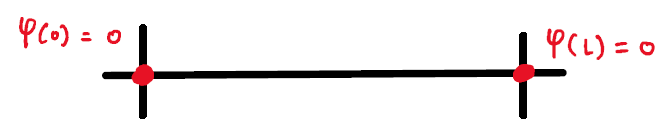
\includegraphics[width=0.8\textwidth]{wave1}\\[1em]
        {\Large $\Downarrow$}\\[1em]
        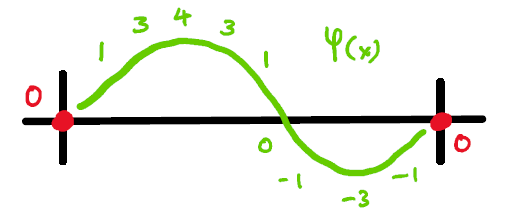
\includegraphics[width=0.6\textwidth]{wave2}
    \end{minipage}
    \hspace{0.01\textwidth}
    \vline
    \hspace{0.01\textwidth}
    \begin{minipage}{0.45\linewidth}
        \centering
        In Poisson equation, 
        boundary conditions are about the line/face at the edge of the region.
        There can be too many variations.\\[1em]
        \begin{minipage}{0.35\linewidth}
            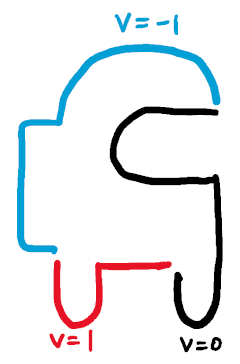
\includegraphics[width=\textwidth]{sus}
        \end{minipage}
        \begin{minipage}{0.45\linewidth}
            {\large \quad$\Rightarrow$\quad $V(\vvec{r})=$\ ?}
        \end{minipage}\\[1ex]
        
        \phantom{abc}
        
    \end{minipage}
\end{center}

\vskip 1em
Even though, we have already seen the solution in one very special case - 
When the \cul[red]{region of} \cul[red]{interest is infinitely large} 
\it{AND} \cul[red]{potential is \bf{chosen} to be $0$ at infinity far}, 
i.e. $V(\vvec{r}=\infty)=0$, 
the solution is exactly the Coulomb's law.
\begin{center}
    \begin{minipage}{0.4\linewidth}
        \aleq{
            \Aboxed{
                V(\red{\vvec{r}}) 
                &= \inv{4\pi\epsilon_0}\underset{\substack{\text{infinitely large}\\\text{space}}}{\iiint}\ 
                    \frac{\rho(\blue{\vvec{r}'})}{\norm{\red{\vvec{r}}-\blue{\vvec{r}'}}}\dd[3]{\blue{\vvec{r}'}}
            }\\[1ex]
            %
            &\sim \inv{4\pi\epsilon_0} \sum_\text{everywhere} \frac{(\text{charge})}{(\text{distance})}\\[1em]
            %
            &\equiv\ \mstack{\text{Coulomb's law for electric potential}\\\scriptsize \text{(But written in a fancier vector form)}}
        }
    \end{minipage}
    \hspace{0.05\textwidth}
    \begin{minipage}{0.25\linewidth}
        \centering
        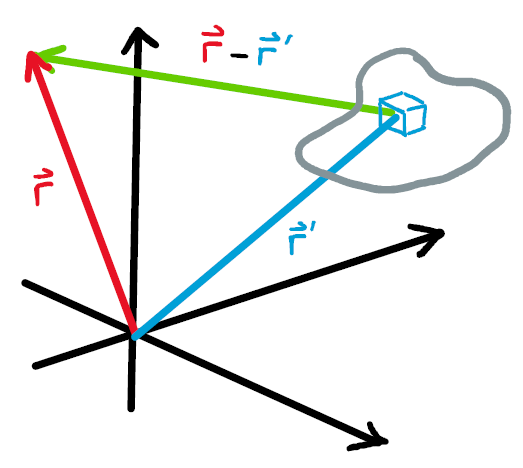
\includegraphics[width=\textwidth]{coulomb_elem}
    \end{minipage}
\end{center}


\newpage
%%%%%%%%%%%%%%
\subsection{Finding $\vvec{E}$ from $Q$}

On the other hand, Poisson equation provides an alternative to calculate E-field distribution from charge distribution.
If we compare the Gauss's law and Poisson equation:
\begin{itemize}
    \item \ul{Poisson equation} : \\[1ex]
    $V(\vvec{r})$ is a scalar function. 
    Only 1 function $V(\vvec{r})$ to be solved.
    \aleq{
        \laplacian V = -\frac{\rho}{\epsilon_0}
        \qquad\Leftrightarrow\qquad
        \cub[blue]{\lapRec{V}}{\text{All about }V} = -\frac{\rho}{\epsilon_0}
    }

    \item \ul{Gauss's law} : \\[1ex] 
    $\vvec{E}(\vvec{r})$ is a vector function with 3 components $E_x(\vvec{r})$, $E_y(\vvec{r})$, $E_z(\vvec{r})$,
    which are \cul[red]{3 inter-depending} functions to be solved.
    \aleq{
        \div \vvec{E} = \frac{\rho}{\epsilon_0}
        \qquad\Leftrightarrow\qquad    
        \cub[red]{\divRec{E_{\cul[red]{x}}}[E_{\cul[red]{y}}][E_{\cul[red]{z}}]}
        {\text{Involve different components}}
         = \frac{\rho}{\epsilon_0}
    }
\end{itemize}

Obviously, there is no reason to try to directly solve the more difficult PDE of $\vvec{E}$
if we can alternatively solve the easier PDE of $V$,
and then take gradient to get $\vvec{E}$ (i.e. via $\vvec{E} = -\grad V$). 

\begin{center}
    \begin{minipage}{0.5\linewidth}
        \centering
        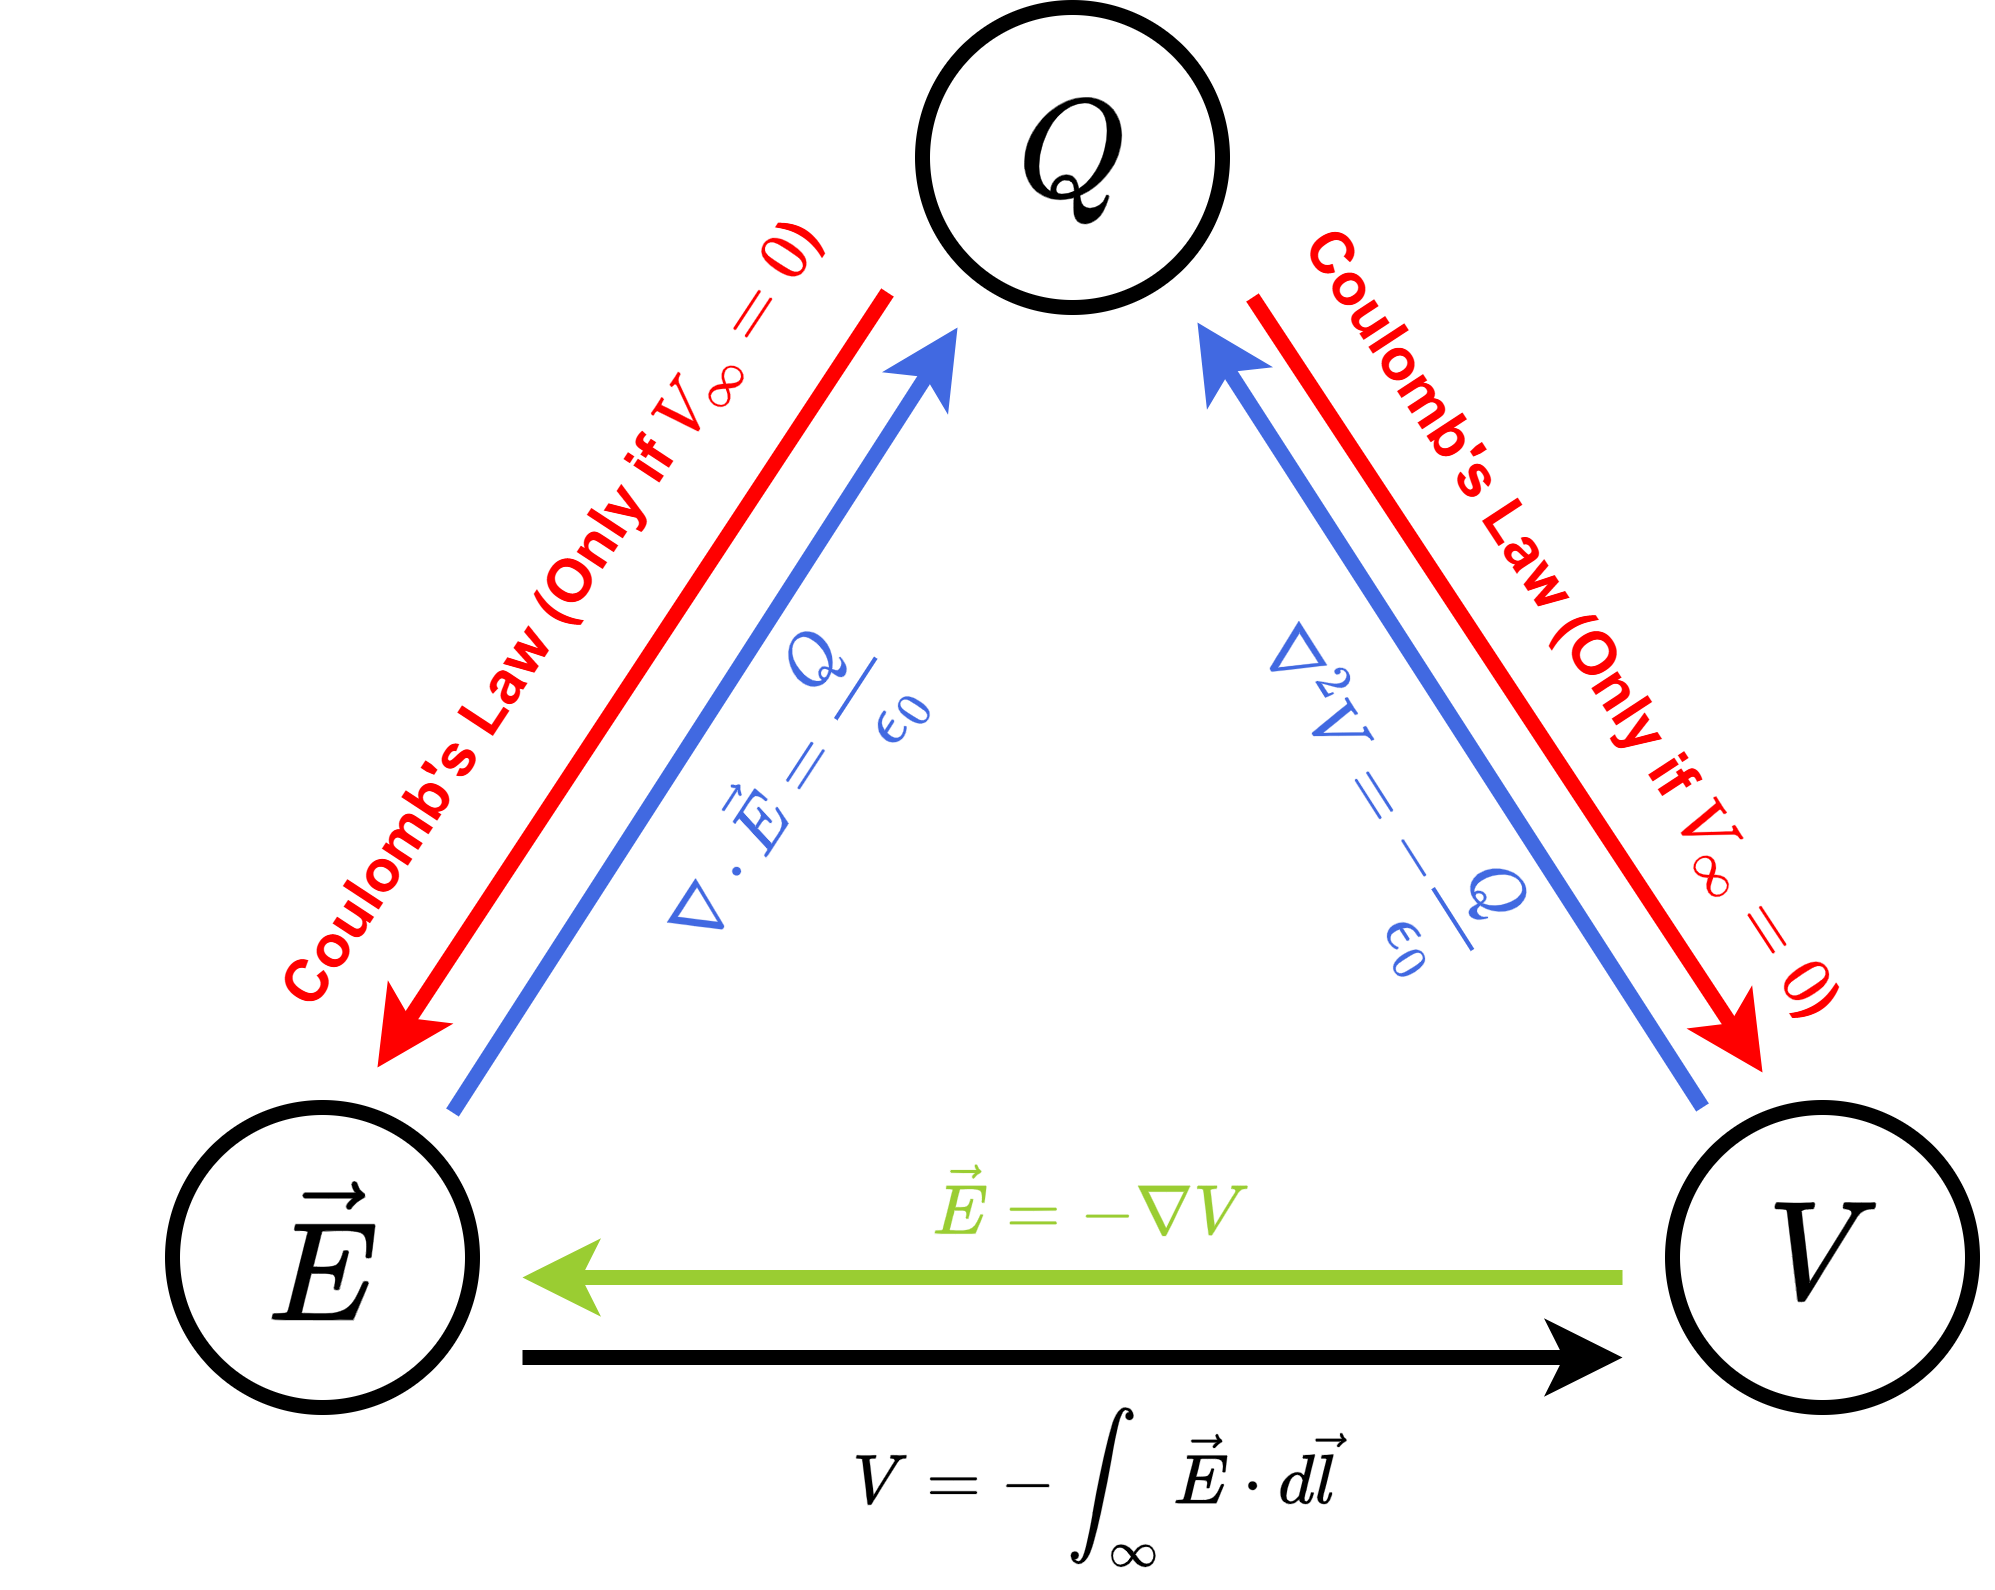
\includegraphics[width=\textwidth]{triangleE}
    \end{minipage}
\end{center}

In this way, we can tell the solution of Gauss's law as a PDE,
which is as expected, the Coulomb's law for $\vvec{E}$.
\aleq{
    \Aboxed{
        \vvec{E}(\red{\vvec{r}}) = - \grad V(\red{\vvec{r}}) 
        &= \inv{4\pi\epsilon_0}\underset{\substack{\text{infinitely large}\\\text{space}}}{\iiint}\ 
            \frac{\rho(\blue{\vvec{r}'})}{\norm{\red{\vvec{r}}-\blue{\vvec{r}'}}^2}
            \qty[\frac{\red{\vvec{r}}-\blue{\vvec{r}'}}{\norm{\red{\vvec{r}}-\blue{\vvec{r}'}}}]\dd[3]{\blue{\vvec{r}'}}
    }\\[1ex]
    %
    &\sim \inv{4\pi\epsilon_0} \sum_\text{everywhere} \frac{(\text{charge})}{(\text{distance})^2} \qty(\substack{\text{unit}\\\text{vector}})\\[1em]
    %
    &\equiv\ \mstack{\text{Coulomb's law for electric field}\\\scriptsize \text{(But written in a fancier vector form)}}
}




\linesep
% Section %%%%%%%%%%%%%%%%%%%%%%%%%%%%%%%%%%%%%%%%%%%%%%%%%%%%
\section{Image Charge Method}

%%%%%%%%%%%%%%
\subsection{Induced Charge \& Equipotential on Conductors}

Suppose we want to solve an electrostatics problem with conductors present.
Because charges can freely flow in conductors,
the presence of external charge sources can \it{induce} new charge in the conductors.
\begin{itemize}
    \item The induced charge's distribution completely depends on the positions of external charge,
    and also the shape of the conductor.

    \item \bf{Measuring the induced charge distribution is impossible}, 
    because any charge probe will disturb it.
\end{itemize}

\begin{center}
    \begin{minipage}{0.16\linewidth}
        \centering
        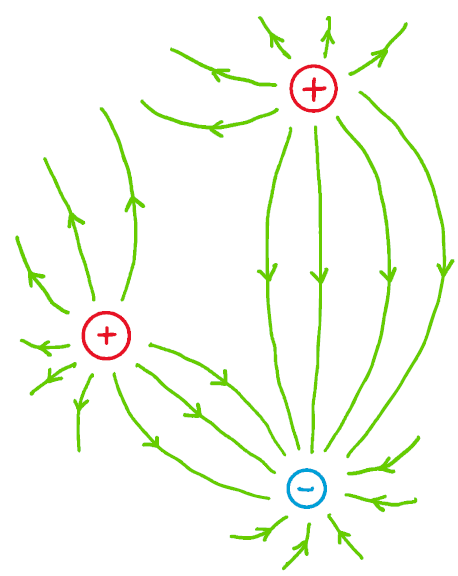
\includegraphics[width=\textwidth]{img_conduct2}
    \end{minipage}
    {\Large \quad$+$\quad}
    \begin{minipage}{0.18\linewidth}
        \centering
        \includegraphics[width=\textwidth]{img_conduct1}
    \end{minipage}
    {\Large \quad$=$\quad}
    \begin{minipage}{0.22\linewidth}
        \centering
        \includegraphics[width=\textwidth]{img_conduct3}
    \end{minipage}
\end{center}

In previous sections, 
we are solving for $\vvec{E}$ and $V$ where the charge distribution $\rho$ is known \cul[red]{everywhere}.
But this time we do not know the exact distribution of induced charge!
Luckily, if the induced charges are distributed on conductors,
there is one property that the induced charges need to satisfy:

\begin{center}
    \begin{minipage}{0.6\textwidth}
        \begin{framed}
            \centering
            Charges on conductor must distribute themselves\\ such that the whole conductor is of equi-potential.
        \end{framed}       
    \end{minipage}
\end{center}

This is intuitive - because charges are allowed to move freely,
they will spontaneously distribute themselves until net electric force on them is $0$,
i.e. the electric potential will be the same everywhere on the conductor.

\begin{center}
    \begin{minipage}{0.25\linewidth}
        \centering
        \red{\footnotesize This charge feels\\[-0.5ex] greater repulsion from\\[-1ex] the right than from the left.}
    \end{minipage}
    \begin{minipage}{0.2\linewidth}
        \centering
        \includegraphics[width=\textwidth]{img_rod1}
    \end{minipage}
    \hspace{0.04\textwidth}
    \vline
    \hspace{0.04\textwidth}
    \begin{minipage}{0.19\linewidth}
        \centering
        \includegraphics[width=\textwidth]{img_rod2}
    \end{minipage}
    \begin{minipage}{0.15\linewidth}
        \centering
        \red{\footnotesize Now the force\\[-1ex] is balanaced.}
    \end{minipage}
\end{center}



%%%%%%%%%%%%%%
\subsection{Image charges}

In the perspective of solving PDE, 
requiring "conductor = equipotential" only means an additional boundary condition of $V$ over the conductor's surface.

\begin{center}
    \begin{minipage}{0.27\linewidth}
        \centering
        \includegraphics[width=\textwidth]{img_bc1}
    \end{minipage}
    {\Large \quad$\equiv$\quad}
    \begin{minipage}{0.27\linewidth}
        \centering
        \includegraphics[width=\textwidth]{img_bc2}
    \end{minipage}
\end{center}

From mathematical studies of Poisson equation,
there is the \bf{uniqueness theorem of Poisson equation} 
(proof on \href{https://en.wikipedia.org/wiki/Uniqueness_theorem_for_Poisson%27s_equation}{wiki}) 
that if the boundary conditions of $V$ is fixed, 
\begin{itemize}
    \item Any solutions of the Poisson equation can only be different by a constant function. 
    \aleq{
        \laplacian V = -\frac{\rho}{\epsilon_0} 
        \qquad\xRightarrow{\text{Solve}}\qquad
        V = V(\vvec{r}) + (\substack{\text{Any constant}\\C})
    }
    \item So E-field, the gradient of $V$, is uniquely determined by the boundary conditions of $V$.
    \aleq{
        \vvec{E}\ =\ -\grad (V(\vvec{r})+C) 
        \ =\ -\grad V(\vvec{r}) + 0 
        \ =\ \qty(\substack{\text{Same for}\\\text{any }C})
    }
\end{itemize}

This theorem allows us to skip calculating where the induced charge are - 
\red{we may find another charge configurations that creates the same potential boundary condition
but easier to calculate.}
By the uniquessness theorem, 
the E-field in these two configurations must be the same.\\

This approach is called the \bf{image charge method},
and the charges that we used to create the alternative configuration are called
\bf{image charge}.
They are called so because the alternative configurations usually look like
a "reflection" of the external charge sources through the conductor surface.


\vskip 2em
\begin{example}
    ("Reflection" by plane)\\

    Consider a point charge \red{$q$} at distance $d$ from an infinitely large metal surface
    which is maintained at $V = 0$.
    We expect an induced charge distribution forming on the surface
    and contribute to the potential/E-field on top of the surface.

    \begin{center}
        \begin{minipage}{0.5\linewidth}
            \centering
            \includegraphics[width=\textwidth]{img_plane1}
        \end{minipage}
    \end{center}

    But we already know another similar configuration that 
    creates a flat equipotential surface of $V=0$ and satisfy $V(\infty=0)$ -
    when there is an additional charge of \blue{$-q$} at distance $d$ under the metal surface.

    \begin{center}
        \begin{minipage}{0.5\linewidth}
            \centering
            \includegraphics[width=\textwidth]{img_plane2}
        \end{minipage}
    \end{center}

    The principle of image charge method tells us that 
    the potential and E-field (on top of the metal surface) in both cases must be identical because 
    they satisfy the same boundary condition of $V$.
    Therefore the potential is 
    \aleq{
        V_{\qty(\substack{\text{top}\\\text{half}})}(x,y,z)
        &= \qty(\mstack{\text{Contribution by}\\\text{original charge }\red{q}}) 
            + \qty(\mstack{\text{Contribution by}\\\text{image charge }\blue{-q}})\\[1ex]
        &= \frac{q}{4\pi\epsilon_0}\inv{\sqrt{x^2+y^2+(z-d)^2}}
            - \frac{q}{4\pi\epsilon_0}\inv{\sqrt{x^2+y^2+(z+d)^2}}
    }

    and the E-field is
    \aleq{
        \vvec{E}_{\qty(\substack{\text{top}\\\text{half}})}(x,y,z) 
            &= -\grad V_{\qty(\substack{\text{top}\\\text{half}})}(x,y,z) \\[1ex]
        &= -\grad \qty(\frac{q}{4\pi\epsilon_0}\qty[\inv{\sqrt{x^2+y^2+(z-d)^2}}
            - \inv{\sqrt{x^2+y^2+(z+d)^2}}])\\[1ex]
        &= \frac{q}{4\pi\epsilon_0} \qty(\frac{x\hhat{x} + y\hhat{y} + (z-d)\hhat{z}}{(x^2+y^2+(z-d)^2)^{\frac{3}{2}}}
            - \frac{x\hhat{x} + y\hhat{y} + (z+d)\hhat{z}}{(x^2+y^2+(z+d)^2)^{\frac{3}{2}}})
    }

    While the $V$ and $\vvec{E}$ on the bottom half must be $0$ because it is in the metal.\\

    After getting $\vvec{E}$, 
    we can also find the induced charge distribution using Gauss's law.
    By drawing a Gaussian box with area $A$ on the surface at position $(x,y,0)$,
    \begin{center}
        \begin{minipage}{0.4\linewidth}
            \aleq{
                \qty(\mstack{\text{Total}\\\text{flux}}) 
                &= \qty(\mstack{\text{Flux through}\\\text{top surface}})\\[1ex]
                &= \vvec{E}_{\qty(\substack{\text{top}\\\text{half}})}(x,y,0) \cdot A\hhat{z}\\[1ex]
                &= \frac{qA}{4\pi\epsilon_0}\frac{-2d}{(x^2+y^2+d^2)^{\frac{3}{2}}}\\[1ex]
                &\equiv \frac{Q_\text{induced}}{\epsilon}
            }
        \end{minipage}
        \hspace{0.05\textwidth}
        \begin{minipage}{0.4\linewidth}
            \centering
            \includegraphics[width=\textwidth]{img_plane3}
        \end{minipage}
    \end{center}
    \aleq{
        \Rightarrow\ \qty(\mstack{\text{Induced charge}\\\text{surface density}})
            = \sigma_{\text{induced}} \equiv \frac{Q_\text{induced}}{A}
        &= -\frac{q}{2\pi}\frac{d}{(x^2+y^2+d^2)^{\frac{3}{2}}}
    }

\end{example}


\vskip 2em
\begin{example}
    ("Reflection" by Sphere)\\

    Consider a point charge \red{$q$} at distance \red{$a$} from the center of a metal sphere of radius $R$
    which is maintained at $V = 0$.
    We expect an induced charge distribution forming on the surface
    and contribute to the potential/E-field on top of the surface.

    \begin{center}
        \begin{minipage}{0.25\linewidth}
            \centering
            \includegraphics[width=\textwidth]{img_sph1}
        \end{minipage}
        \qquad$\Rightarrow$\qquad
        \begin{minipage}{0.25\linewidth}
            \centering
            \includegraphics[width=\textwidth]{img_sph2}
        \end{minipage}
    \end{center}

    In the spherical case,
    we can substitute the induced charge by a single point charge \blue{$-q'$} 
    at distance \blue{$b$} from the sphere's center,
    which can be calculated by 
    

    \begin{center}
        \begin{minipage}{0.4\linewidth}
            \aleq{
                \Aboxed{
                    \bcase{
                        \blue{b} &= \frac{R^2}{\red{a}}\\
                        \blue{q'} &= -\frac{R}{\red{a}}q
                    }
                }
            }
        \end{minipage}
        \hspace{0.05\textwidth}
        \begin{minipage}{0.25\linewidth}
            \centering
            \includegraphics[width=\textwidth]{img_sph3}
        \end{minipage}
    \end{center}

    %%%%%
    \vskip 0.5em
    \underline{\textit{Proof}}\par
    \hspace{0.025\textwidth}\begin{minipage}{0.95\linewidth}
    \vskip 0.5em

        Choose the origin to be the center of the sphere and 
        direction to \red{$q$} to be $\theta=0$.
        Since it requires the potential on the sphere to be $V(r=R)=0$,
        we can write the total $V$ as 
        \aleq{
            V(R, \theta, \phi) = 0 
            &= \qty(\mstack{\text{Contribution by}\\\text{original charge }\red{q}}) 
                + \qty(\mstack{\text{Contribution by}\\\text{image charge }\blue{-q'}})\\[1ex]
            &= \frac{\red{q}}{4\pi\epsilon_0}\inv{\sqrt{R^2 + \red{a}^2-2R\red{a}\cos\theta}}
                - \frac{\blue{q'}}{4\pi\epsilon_0}\inv{\sqrt{R^2 + \blue{b}^2-2R\blue{b}\cos\theta}}\\[2ex]
            \Rightarrow\quad \qty(\frac{-q'}{q}) &= 
                \frac{R^2+b^2-2Rb\cos\theta}{R^2+a^2-2Ra\cos\theta}\\[1ex]
            0 &= \cub[yellow]{\qty[1-\qty(\frac{q'}{q})^2]R^2 
                + \qty[b^2 - \qty(\frac{q'}{q})^2a^2]}{\text{This part is independent of }\theta}
                - \cub[green]{2R \qty[b - \qty(\frac{q'}{q})^2a]}{\text{Coefficient of }\cos\theta}\cos\theta
        }

        This relation should hold for any $\theta$.
        \begin{enumerate}
            \item Therefore the coefficient of $\cos\theta$ must be $0$.
            \aleq{
                0 &= 2R \qty[b - \qty(\frac{q'}{q})^2a]\\
                \Rightarrow\quad \frac{b}{a} &= \qty(\frac{q'}{q})^2 
            }

            \item Then the remaining term must also become $0$. 
            \aleq{
                0 &= \qty[1-\qty(\frac{q'}{q})^2]R^2 + \qty[b^2 - \qty(\frac{q'}{q})^2a^2]\\
                &= \qty(1-\frac{b}{a})R^2 + \qty(b^2 - a^2\cdot\frac{b}{a})\\
                &= \qty(1-\frac{b}{a})R^2 + ab\qty(\frac{b}{a} - 1)\\
                &= \qty(1-\frac{b}{a})\qty(R^2-ab)\\
                \Rightarrow\quad \text{Either}&\quad b=a_\text{\scriptsize \ (reject)} 
                \quad\text{or}\quad \cul[red]{b=\frac{R^2}{a}}
            }
        \end{enumerate}
    
    \end{minipage}
    \vskip 1.5em \par

    \hspace{0.025\textwidth}\begin{minipage}{0.95\linewidth}

        Finally substitute back into $\frac{b}{a} = \qty(\frac{q'}{q})^2$ to get 
        \aleq{
            q' = \pm \sqrt{\frac{b}{a}}q = \tkn{image_minus}{\red{-}}\frac{R}{a}q
        }
        \addArrow[red]{image_minus}{(0,-4.5ex)}
        {\scriptsize The image charge must be\\[-1ex]\scriptsize negative to be physical}
        {(0,-0.5ex)}{(0,-1ex)}

    \hfill $\square$
    \end{minipage}
    \vskip 1.5em \par

\end{example}


\vskip 2em
\begin{exercise}
    How do you add image charges in these situations,
    such that the potential on the metal surface satisfy $V=0$?

    \begin{center}
        \begin{minipage}{0.3\linewidth}
            \centering
            \includegraphics[width=0.6\textwidth]{img_ex1}
        \end{minipage}
        \hspace{0.05\textwidth}
        \begin{minipage}{0.3\linewidth}
            \centering
            \includegraphics[width=\textwidth]{img_ex2}
        \end{minipage}
    \end{center}

    \vskip 1em
    \bf{\ul{Solutions}}:

    \begin{center}
        \begin{minipage}{0.3\linewidth}
            \centering
            \includegraphics[width=0.8\textwidth]{img_ex1s}
        \end{minipage}
        \hspace{0.08\textwidth}
        \begin{minipage}{0.3\linewidth}
            \centering
            \includegraphics[width=\textwidth]{img_ex2s}
        \end{minipage}
        \hspace{0.03\textwidth}
    \end{center}

\end{exercise}

\vskip 1em
\linesep
%%%%%%%%%%%%%%
Here we shall summarize the methods of solving electrostatics problems:
\begin{enumerate}
    \item Very symmetric configurations 
    $\Rightarrow$ Gauss's law integral form. No calculus required.

    \item Not so symmetric but satisfies $V(\vvec{r}=\infty)=0$ 
    $\Rightarrow$ Multiple integral with Coulomb's law.

    \item $V(\vvec{r})=0$ on some nice surfaces with induced charge
    $\Rightarrow$ Try image charge method.

    \item All the above do not apply 
    $\Rightarrow$ Solve Poisson equation of $V(\vvec{r})$ explicitly. PDE hell. %\emoji{skull}
\end{enumerate}
\linesep
%%%
\theend
\end{document}